% =============================================================================
% Regime-Dependent Delta Hedging with SVI-Calibrated Volatility Surfaces:
% An Empirical Analysis of SPX Index Options
% =============================================================================
% Zaid Annigeri — Master of Quantitative Finance, Rutgers Business School
% =============================================================================

\documentclass[12pt, letterpaper]{article}

% --- Page geometry ---
\usepackage[margin=1in]{geometry}

% --- Encoding and fonts ---
\usepackage[utf8]{inputenc}
\usepackage[T1]{fontenc}
\usepackage{lmodern}

% --- Math ---
\usepackage{amsmath, amssymb, amsthm}
\usepackage{mathtools}

% --- Tables ---
\usepackage{booktabs}
\usepackage{tabularx}
\usepackage{multirow}
\usepackage{array}

% --- Figures ---
\usepackage{graphicx}
\usepackage{float}
\usepackage{subcaption}

% --- Colors and hyperlinks ---
\usepackage[dvipsnames]{xcolor}
\usepackage[colorlinks=true, linkcolor=NavyBlue, citecolor=NavyBlue, urlcolor=NavyBlue]{hyperref}

% --- Bibliography ---
\usepackage[round, sort&compress]{natbib}

% --- Spacing ---
\usepackage{setspace}
\onehalfspacing

% --- Headers ---
\usepackage{fancyhdr}
\setlength{\headheight}{14.5pt}
\pagestyle{fancy}
\fancyhf{}
\rhead{\thepage}
\lhead{\nouppercase{\leftmark}}
\renewcommand{\headrulewidth}{0.4pt}

% --- Captions ---
\usepackage[font=small, labelfont=bf]{caption}

% --- Enumeration ---
\usepackage{enumitem}

% --- Custom commands ---
\newcommand{\E}{\mathbb{E}}
\newcommand{\Var}{\text{Var}}
\newcommand{\Cov}{\text{Cov}}
\newcommand{\Corr}{\text{Corr}}
\newcommand{\diff}{\,\mathrm{d}}
\newcommand{\bps}{\,\text{bps}}
\newcommand{\ie}{\textit{i.e.}}
\newcommand{\eg}{\textit{e.g.}}

% --- Theorem-like environments ---
\newtheorem{hypothesis}{Hypothesis}

% --- Graphics path ---
\graphicspath{{../results/figures/}}

% =============================================================================
\begin{document}

% --- Title page ---
\begin{titlepage}
\centering
\vspace*{2cm}

{\LARGE\bfseries Regime-Dependent Delta Hedging with\\[0.3cm]
SVI-Calibrated Volatility Surfaces:\\[0.3cm]
An Empirical Analysis of SPX Index Options\par}

\vspace{2cm}

{\Large Zaid Annigeri\par}

\vspace{1cm}

{\large
A thesis submitted in partial fulfillment of the requirements\\
for the degree of\\[0.5cm]
\textbf{Master of Quantitative Finance}\\[0.5cm]
Rutgers Business School\\
Rutgers, The State University of New Jersey\par}

\vspace{2cm}

{\large October 2025 -- March 2026\par}

\vfill

\end{titlepage}

% --- Abstract ---
\newpage
\thispagestyle{plain}
\begin{center}
{\Large\bfseries Abstract}
\end{center}

\noindent
This thesis investigates which volatility input minimizes delta-hedging error for S\&P~500 index options across different market regimes. I compare five volatility inputs for computing Black--Scholes hedge deltas: (1)~flat at-the-money implied volatility, (2)~strike-specific implied volatility from a calibrated Gatheral SVI surface, (3)~21-day close-to-close realized volatility, (4)~21-day Parkinson realized volatility, and (5)~21-day Yang--Zhang realized volatility. Using OptionMetrics data on 2,000 stratified SPX options from January 2019 through December 2024, I conduct daily-rebalanced delta-hedging backtests across four VIX-defined regimes (Low, Normal, High, and Crisis).

The results challenge prevailing intuition. Aggregate hedging performance ranks close-to-close realized volatility first, with a statistically significant 5.8\% reduction in hedging error standard deviation versus the flat BSM benchmark ($F = 0.89$, $p = 0.008$). The SVI surface, despite achieving a median calibration RMSE of 19.5 basis points and 68.6\% butterfly arbitrage-free rate, \textit{increases} hedging error variance by 9.4\% overall. However, the optimal volatility input is regime- and moneyness-dependent: SVI dominates for out-of-the-money calls (RMSE reductions of 6--12\% versus flat BSM), while realized volatility estimators outperform for out-of-the-money puts. An El~Karoui--style P\&L decomposition reveals that higher-order residuals (vanna, volga, jumps) dominate variance attribution across all regimes (153--162\%), while discrete rebalancing error and volatility misspecification contribute negatively through the gamma--theta offset.

These findings suggest that the calibration noise introduced by SVI fitting outweighs its informational benefit for most option types, but that a regime-conditional approach selecting different volatility inputs by moneyness and VIX level could improve hedging outcomes relative to any single-input strategy.

\vspace{0.5cm}
\noindent\textbf{Keywords:} delta hedging, implied volatility surface, SVI parameterization, realized volatility, VIX regimes, hedging error, SPX options, P\&L decomposition

% --- Table of Contents ---
\newpage
\tableofcontents
\newpage
\listoftables
\listoffigures
\newpage

% =============================================================================
% CHAPTER 1: INTRODUCTION
% =============================================================================
\section{Introduction}
\label{sec:introduction}

Every trading day, options desks face a deceptively simple question: which volatility should we use to compute our hedge ratios? The Black--Scholes--Merton framework \citep{Black1973, Merton1973} provides a clean answer---use the true volatility of the underlying---but this parameter is unobservable. In practice, traders must choose among imperfect proxies: the option's own implied volatility, a flat at-the-money (ATM) implied volatility, a calibrated volatility surface, or some estimate of realized volatility. The wrong choice costs money.

This question matters more than it might seem. A delta-hedging program that uses a volatility input misaligned with the true dynamics of the underlying will systematically accumulate hedging errors. These errors manifest as unexplained P\&L variance, which risk managers must reserve against and which erodes trading desk profitability. While the theoretical properties of delta hedging under misspecified volatility are well understood \citep{ElKaroui1998}, the empirical question---which volatility input actually minimizes hedging error on real options---has received surprisingly little attention.

The Stochastic Volatility Inspired (SVI) parameterization \citep{Gatheral2004, Gatheral2014} has become the industry standard for fitting implied volatility surfaces. It captures the volatility smile with five intuitive parameters and admits analytical derivatives that make it computationally attractive. A substantial literature validates SVI's calibration quality: typical root-mean-square errors of 10--50 basis points for liquid equity index options. Yet this literature stops at calibration. No study, to my knowledge, has tested whether feeding SVI-calibrated implied volatilities into a delta-hedging program actually produces better hedging outcomes than simpler alternatives.

This gap is the starting point for my thesis. I conduct a large-scale empirical experiment comparing five volatility inputs for delta hedging S\&P~500 index options:

\begin{enumerate}[label=(\arabic*)]
    \item \textbf{Flat BSM IV}: the at-the-money implied volatility for the relevant expiry, applied to all strikes.
    \item \textbf{SVI Surface IV}: the strike-specific implied volatility from a Gatheral raw SVI calibration.
    \item \textbf{Close-to-Close RV}: 21-day close-to-close realized volatility of the SPX index.
    \item \textbf{Parkinson RV}: 21-day Parkinson (high--low range) realized volatility.
    \item \textbf{Yang--Zhang RV}: 21-day Yang--Zhang (OHLC) realized volatility.
\end{enumerate}

I structure the empirical analysis around three hypotheses:

\begin{hypothesis}
\label{hyp:svi}
SVI surface implied volatility reduces delta-hedging error variance relative to flat BSM implied volatility, because strike-specific volatilities capture smile dynamics that a flat input ignores.
\end{hypothesis}

\begin{hypothesis}
\label{hyp:yz}
The Yang--Zhang realized volatility estimator outperforms the close-to-close estimator as a hedging input, because its higher statistical efficiency (incorporating open, high, low, and close prices) provides a more accurate estimate of current volatility.
\end{hypothesis}

\begin{hypothesis}
\label{hyp:regime}
The optimal volatility input is regime-dependent: SVI surface IV dominates in calm markets where the smile is stable and well-estimated, while realized volatility dominates in crisis periods when implied surfaces are noisy and mean-reverting dynamics favor backward-looking estimators.
\end{hypothesis}

The experiment uses OptionMetrics IvyDB data on SPX options from January 2019 through December 2024---a period that includes the COVID-19 crash, the 2022 rate-hiking cycle, and extended low-volatility regimes. I sample 2,000 options stratified across four VIX-defined market regimes, hedge each daily to expiry using each of the five volatility inputs, and analyze the resulting P\&L distributions. I complement the hedging analysis with an El~Karoui decomposition of hedging P\&L into discrete rebalancing error, volatility misspecification, and higher-order residual components, and I validate the SVI calibration using the Durrleman butterfly arbitrage condition.

The results are nuanced and, in several respects, surprising. They challenge the assumption that more information (a full volatility surface) necessarily translates into better hedging. The remainder of this thesis is organized as follows. Section~\ref{sec:literature} reviews the relevant literature. Section~\ref{sec:methodology} presents the methodology. Section~\ref{sec:data} describes the data. Section~\ref{sec:results} reports the empirical results. Section~\ref{sec:discussion} discusses implications for practitioners. Section~\ref{sec:conclusion} concludes.


% =============================================================================
% CHAPTER 2: LITERATURE REVIEW
% =============================================================================
\section{Literature Review}
\label{sec:literature}

This thesis sits at the intersection of four research streams: (1)~Black--Scholes hedging and its limitations, (2)~advanced delta-hedging methods, (3)~the SVI volatility surface parameterization, and (4)~realized volatility estimation. I review each in turn before identifying the gap that motivates this study.

\subsection{Black--Scholes Hedging and Its Limitations}

The Black--Scholes--Merton framework \citep{Black1973, Merton1973} remains the foundation of options hedging despite its well-known limitations. Under the model's assumptions---constant volatility, continuous trading, no transaction costs, and geometric Brownian motion---the option price is a deterministic function of the underlying price, time, and a single volatility parameter. The hedge ratio (delta) is the partial derivative of the option price with respect to the underlying:
\begin{equation}
    \Delta_{\text{call}} = e^{-qT} N(d_1), \qquad \Delta_{\text{put}} = e^{-qT} [N(d_1) - 1],
    \label{eq:bsm_delta}
\end{equation}
where $d_1 = [\ln(S/K) + (r - q + \tfrac{1}{2}\sigma^2)T] / (\sigma\sqrt{T})$ and $N(\cdot)$ is the standard normal CDF.

In practice, every assumption is violated. Volatility is stochastic, trading is discrete, and transaction costs are non-zero. The seminal contribution of \citet{ElKaroui1998} established that the Black--Scholes hedge is surprisingly robust to volatility misspecification: if the hedging volatility $\sigma_h$ dominates the realized volatility path almost surely, then the hedging portfolio produces a non-negative terminal P\&L for the option seller. This ``robustness under domination'' result provides theoretical grounding for the common practice of hedging with implied (rather than realized) volatility, since implied volatility typically exceeds realized volatility due to the variance risk premium.

\citet{Hull2018} provides a comprehensive treatment of the practical aspects of delta hedging, including the effects of discrete rebalancing and the gamma--theta tradeoff. The key insight is that delta-hedging error over a discrete time interval $\Delta t$ is approximately
\begin{equation}
    \epsilon_t \approx \frac{1}{2}\Gamma_t \left[(\Delta S_t)^2 - \sigma_h^2 S_t^2 \Delta t\right],
    \label{eq:discrete_error}
\end{equation}
which has zero expectation under the hedging measure but non-zero variance. This variance is the ``cost of discrete hedging'' and is proportional to $\Gamma^2$ and the kurtosis of returns.

\subsection{Advanced Delta-Hedging Methods}

Several authors have proposed modifications to the standard BSM delta to improve hedging performance. \citet{Hull2017} introduced the \textit{minimum-variance delta}, which adjusts the BSM delta to account for the empirical relationship between implied volatility movements and underlying price changes. Their key metric is the ``Gain'' statistic:
\begin{equation}
    \text{Gain} = 1 - \frac{\text{Std}(\text{hedge error under method } i)}{\text{Std}(\text{hedge error under flat BSM})},
    \label{eq:gain}
\end{equation}
which measures the percentage reduction in hedging error standard deviation relative to the flat BSM benchmark. A positive Gain indicates improvement. \citet{Hull2017} report Gains of 2--10\% for their minimum-variance approach on S\&P~500 options, with larger improvements for out-of-the-money options.

\citet{Alexander2012} examine regime-dependent smile-adjusted deltas, showing that the optimal hedge ratio depends on the prevailing volatility regime. In high-volatility environments, the smile steepens and becomes less stable, making smile-based adjustments less reliable. Their work suggests that the benefit of incorporating smile information into hedge ratios may be conditional on market conditions---a hypothesis I test directly.

\citet{Taleb1997} provides practitioner-oriented insights on the challenges of dynamic hedging, emphasizing that the gap between theoretical continuous-time hedging and practical discrete rebalancing is often larger than model risk from volatility misspecification.

\subsection{The SVI Parameterization}

\citet{Gatheral2004} introduced the Stochastic Volatility Inspired (SVI) parameterization for the implied variance smile. The raw SVI parameterization expresses total implied variance $w(k) = \sigma^2_{\text{BS}}(k) \cdot T$ as a function of log-moneyness $k = \ln(K/F)$:
\begin{equation}
    w(k) = a + b\left[\rho(k - m) + \sqrt{(k - m)^2 + \sigma^2}\right],
    \label{eq:svi}
\end{equation}
where $a$ controls the overall variance level, $b$ scales the wings, $\rho \in (-1, 1)$ controls the skew, $m$ shifts the smile center, and $\sigma > 0$ controls curvature. The parameterization is ``inspired'' by stochastic volatility models in the sense that its asymptotic behavior matches the large-strike behavior of the Heston model.

\citet{Gatheral2014} refined the SVI framework, establishing necessary and sufficient conditions for the absence of butterfly (static) arbitrage. The key condition, due to \citet{Durrleman2005}, requires that the density function implied by the total variance surface remain non-negative everywhere:
\begin{equation}
    g(k) = \left(1 - \frac{k\, w'(k)}{2\, w(k)}\right)^2 - \frac{[w'(k)]^2}{4}\left(\frac{1}{w(k)} + \frac{1}{4}\right) + \frac{w''(k)}{2} \geq 0
    \label{eq:durrleman}
\end{equation}
for all $k$, where primes denote derivatives with respect to $k$.

A significant body of work addresses SVI calibration methodology. Two-stage approaches combining global optimization (differential evolution) with local refinement (L-BFGS-B, Levenberg--Marquardt) are standard \citep{Storn1997}. Typical calibration quality for liquid equity index options ranges from 10 to 50 basis points RMSE in implied volatility terms.

Crucially, the entire SVI literature focuses on calibration quality---how well the parameterization fits observed implied volatilities. \textbf{No study, to my knowledge, has tested whether SVI-calibrated implied volatilities produce better delta-hedging outcomes than simpler alternatives.} This is the central gap my thesis addresses.

\subsection{Realized Volatility Estimators}

The finance literature offers several estimators of realized volatility, differing in which price information they incorporate and in their statistical efficiency.

The \textit{close-to-close} estimator is the standard deviation of log returns, annualized by $\sqrt{252}$. It uses only closing prices and is the most common benchmark. \citet{Parkinson1980} proposed a range-based estimator using daily high and low prices:
\begin{equation}
    \hat{\sigma}_P^2 = \frac{1}{4 \ln 2} \cdot \frac{1}{n} \sum_{i=1}^{n} \left[\ln\left(\frac{H_i}{L_i}\right)\right]^2,
    \label{eq:parkinson}
\end{equation}
which is approximately 5 times more efficient than the close-to-close estimator under geometric Brownian motion.

\citet{Yang2000} developed a drift-independent estimator that combines overnight, open-to-close, and range-based components using all four OHLC prices:
\begin{equation}
    \hat{\sigma}_{\text{YZ}}^2 = \hat{\sigma}_{\text{overnight}}^2 + k \cdot \hat{\sigma}_{\text{open-close}}^2 + (1 - k) \cdot \hat{\sigma}_{\text{RS}}^2,
    \label{eq:yangzhang}
\end{equation}
where $k = 0.34 / (1.34 + (n+1)/(n-1))$ and $\hat{\sigma}_{\text{RS}}^2$ is the Rogers--Satchell range-based variance. The Yang--Zhang estimator is unbiased for processes with drift and achieves higher efficiency than both the close-to-close and Parkinson estimators.

\citet{Shu2006} provide a comprehensive comparison of range-based volatility estimators, finding that the Yang--Zhang estimator has the lowest mean squared error among OHLC-based estimators for typical equity data. However, their comparison is on \textit{forecasting} accuracy, not \textit{hedging} outcomes. Whether a more efficient volatility estimator translates into better hedging performance is an open empirical question.

\subsection{The Gap}

The literature reveals a clear gap at the intersection of these four streams. SVI calibration research stops at fitting quality. Realized volatility research stops at forecasting accuracy. Delta-hedging research either uses stylized simulations or tests a narrow set of volatility inputs. No study brings all three together to ask: \textit{across different market regimes and option moneyness levels, which volatility input---flat implied, smile-calibrated implied, or realized---actually minimizes delta-hedging error for real SPX options?} This thesis provides the first empirical answer.


% =============================================================================
% CHAPTER 3: METHODOLOGY
% =============================================================================
\section{Methodology}
\label{sec:methodology}

This section describes the computational infrastructure and statistical methods used in the empirical analysis. The framework was implemented in Python, with all code written as standalone functions for transparency and reproducibility.

\subsection{Pricing Framework}
\label{sec:pricing}

The core pricing engine implements the Black--Scholes--Merton model with continuous dividend yield $q$. For a European call option:
\begin{equation}
    C = S \, e^{-qT} N(d_1) - K \, e^{-rT} N(d_2),
    \label{eq:bs_call}
\end{equation}
\begin{equation}
    d_1 = \frac{\ln(S/K) + (r - q + \tfrac{1}{2}\sigma^2)T}{\sigma\sqrt{T}}, \qquad d_2 = d_1 - \sigma\sqrt{T},
    \label{eq:d1d2}
\end{equation}
where $S$ is the spot price, $K$ the strike price, $T$ the time to expiry, $r$ the risk-free rate, $q$ the continuous dividend yield (set to 1.3\% for SPX), and $\sigma$ the volatility input. Put prices follow by put-call parity or directly from the BSM formula with $N(-d_1)$ and $N(-d_2)$.

The implementation supports Cox--Ross--Rubinstein binomial pricing (1,000 steps) and Monte Carlo simulation (500,000 paths with antithetic variates and control variate variance reduction) for validation purposes. Cross-method pricing differences are below 0.01\% for the European options in this study.

\subsection{Greeks Computation}
\label{sec:greeks}

Eight analytical Greeks are computed from the BSM model: delta, gamma, vega, theta, rho, vanna, volga, and charm. For the hedging backtest, the key Greeks are delta:
\begin{equation}
    \Delta_{\text{call}} = e^{-qT} N(d_1), \qquad \Delta_{\text{put}} = e^{-qT}[N(d_1) - 1],
    \label{eq:delta}
\end{equation}
and gamma:
\begin{equation}
    \Gamma = \frac{e^{-qT}\, n(d_1)}{S \, \sigma \sqrt{T}},
    \label{eq:gamma}
\end{equation}
where $n(\cdot)$ is the standard normal PDF. Gamma is used in the P\&L decomposition (Section~\ref{sec:pnl_decomp}). All Greeks are validated against finite-difference approximations with errors below 0.1\%.

\subsection{SVI Calibration Pipeline}
\label{sec:svi_calibration}

\subsubsection{Gatheral Raw SVI Parameterization}

I use Gatheral's raw SVI parameterization \citep{Gatheral2004}, which models total implied variance as a function of log-moneyness $k = \ln(K/F)$, where $F = S \cdot e^{(r-q)T}$ is the forward price:
\begin{equation}
    w(k) = a + b\left[\rho(k - m) + \sqrt{(k - m)^2 + \sigma^2}\right].
    \label{eq:svi_raw}
\end{equation}
The implied volatility at strike $K$ and expiry $T$ is recovered as $\sigma_{\text{BS}}(K, T) = \sqrt{w(k) / T}$.

\subsubsection{Three-Stage Optimization}

Each (date, expiry) slice is calibrated independently using a three-stage optimization pipeline that balances speed with quality:

\begin{enumerate}
    \item \textbf{Least-squares warm start.} Trust-region reflective (TRF) least squares minimizes $\sum_i [w_{\text{SVI}}(k_i) - w_{\text{market},i}]^2$ with initial guess $x_0 = [\hat{w}_{\text{ATM}}, 0.1, -0.3, 0.0, 0.1]$ and box constraints. Maximum 200 function evaluations.

    \item \textbf{Differential evolution (DE).} The least-squares solution seeds a short DE run \citep{Storn1997} with population size 5, 15 generations, and fixed random seed 42 for reproducibility. This provides global search capability while keeping computation under 200~ms per slice.

    \item \textbf{L-BFGS-B polish.} The DE solution is refined with bounded quasi-Newton optimization to achieve local optimality.
\end{enumerate}

Parameter bounds are $a \in [-0.5, 0.5]$, $b \in [0.001, 2.0]$, $\rho \in [-0.99, 0.99]$, $m \in [-0.5, 0.5]$, and $\sigma \in [0.001, 2.0]$. Slices with fewer than 5 strikes or RMSE exceeding 300 basis points are rejected. If the initial pipeline yields RMSE above 200~bps, three alternative starting points with different skew initializations ($\rho_0 \in \{-0.5, 0.0, -0.7\}$) are attempted.

\subsubsection{Calibration Thinning and Interpolation}

To make the calibration tractable over a six-year sample, I calibrate every 5th trading day per expiry date (plus the first and last dates), yielding approximately 3,130 calibration points from the full set of over 12,500 unique (date, expiry) slices. SVI parameters for non-calibrated dates are obtained by linear interpolation of each parameter along the date axis, holding the expiry fixed. This approach assumes smooth evolution of the smile shape between calibration dates.

\subsubsection{SVI IV Application Guards}

To prevent pathological SVI-implied volatilities from corrupting the hedging backtest, I apply two guards:
\begin{enumerate}
    \item \textbf{Range guard:} SVI IV must satisfy $0.01 \leq \sigma_{\text{SVI}} \leq 3.0$.
    \item \textbf{Deviation guard:} $|\sigma_{\text{SVI}} - \sigma_{\text{market}}| \leq 0.05$ (5 volatility points).
\end{enumerate}
Observations violating either guard fall back to the market implied volatility.

\subsubsection{Butterfly Arbitrage Validation}

I validate each calibrated SVI slice using the \citet{Durrleman2005} condition (Equation~\ref{eq:durrleman}). The analytical derivatives of the raw SVI are:
\begin{align}
    w'(k) &= b\left[\rho + \frac{k - m}{\sqrt{(k - m)^2 + \sigma^2}}\right], \label{eq:svi_wprime} \\
    w''(k) &= \frac{b\, \sigma^2}{\left[(k - m)^2 + \sigma^2\right]^{3/2}}. \label{eq:svi_wdoubleprime}
\end{align}
I evaluate $g(k)$ on a grid of 201 evenly spaced points in $k \in [-0.5, 0.5]$ and flag a slice as containing butterfly arbitrage if $\min_k g(k) < -10^{-10}$.

\subsection{Realized Volatility Estimators}
\label{sec:rv_estimators}

All three estimators use a 21-trading-day rolling window and are annualized by $\sqrt{252}$.

\subsubsection{Close-to-Close}

The standard estimator based on log returns $r_t = \ln(C_t / C_{t-1})$:
\begin{equation}
    \hat{\sigma}_{\text{CC}} = \sqrt{\frac{252}{n-1} \sum_{i=1}^{n} (r_i - \bar{r})^2}.
    \label{eq:rv_cc}
\end{equation}

\subsubsection{Parkinson}

The range-based estimator using daily high ($H$) and low ($L$) prices \citep{Parkinson1980}:
\begin{equation}
    \hat{\sigma}_P = \sqrt{\frac{252}{4n\ln 2} \sum_{i=1}^{n} \left[\ln\left(\frac{H_i}{L_i}\right)\right]^2}.
    \label{eq:rv_park}
\end{equation}
Under GBM, this is approximately 5 times more statistically efficient than close-to-close.

\subsubsection{Yang--Zhang}

The drift-independent OHLC estimator \citep{Yang2000} decomposes variance into overnight, open-to-close, and intraday range components:
\begin{align}
    \hat{\sigma}_{\text{YZ}}^2 &= \hat{\sigma}_{\text{overnight}}^2 + k \cdot \hat{\sigma}_{\text{OC}}^2 + (1 - k) \cdot \hat{\sigma}_{\text{RS}}^2, \label{eq:rv_yz} \\
    k &= \frac{0.34}{1.34 + \frac{n + 1}{n - 1}}, \nonumber
\end{align}
where $\hat{\sigma}_{\text{overnight}}^2$ is the variance of $\ln(O_t / C_{t-1})$, $\hat{\sigma}_{\text{OC}}^2$ is the variance of $\ln(C_t / O_t)$, and $\hat{\sigma}_{\text{RS}}^2$ is the Rogers--Satchell range-based variance:
\begin{equation}
    \hat{\sigma}_{\text{RS}}^2 = \frac{1}{n}\sum_{i=1}^{n}\left[\ln\frac{H_i}{O_i}\cdot\ln\frac{H_i}{C_i} + \ln\frac{L_i}{O_i}\cdot\ln\frac{L_i}{C_i}\right].
    \label{eq:rogers_satchell}
\end{equation}
The resulting estimator is annualized by multiplying by 252.

\subsection{Delta-Hedging Backtest Protocol}
\label{sec:hedging_protocol}

\subsubsection{Setup}

For each sampled option, I simulate selling one contract and delta-hedging it daily from entry to expiry. At each rebalancing date $t$, the hedge position in the underlying is set to $\Delta_t(\sigma_h)$, where $\sigma_h$ is the volatility input for that method. The hedging error (P\&L) for one option is:
\begin{equation}
    \text{Hedge Error} = \sum_{t=0}^{N-1} \left[\Delta_t(\sigma_h) \cdot (S_{t+1} - S_t) - (V_{t+1} - V_t)\right],
    \label{eq:hedge_error}
\end{equation}
where $V_t$ is the market price of the option at time $t$. This measures the difference between what the hedge portfolio earned and what the option liability changed by. A perfect hedge yields zero.

\subsubsection{Volatility Inputs}

Each option is hedged five times, once with each volatility input:

\begin{itemize}
    \item \textbf{Flat BSM IV ($\sigma_{\text{ATM}}$):} The implied volatility of the option closest to ATM (moneyness nearest 1.0) for the same date and expiry. This is constant across strikes but varies daily.
    \item \textbf{SVI Surface IV ($\sigma_{\text{SVI}}$):} The implied volatility interpolated from the calibrated SVI surface at the option's own strike and expiry. This varies across both strikes and dates.
    \item \textbf{Close-to-Close RV ($\hat{\sigma}_{\text{CC}}$):} The 21-day rolling close-to-close realized volatility of the SPX index on date $t$. This is the same for all options on a given date.
    \item \textbf{Parkinson RV ($\hat{\sigma}_P$):} The 21-day rolling Parkinson realized volatility.
    \item \textbf{Yang--Zhang RV ($\hat{\sigma}_{\text{YZ}}$):} The 21-day rolling Yang--Zhang realized volatility.
\end{itemize}

\subsubsection{Sample Selection}

Options must satisfy the following criteria to be included:

\begin{itemize}
    \item DTE at entry between 14 and 90 calendar days.
    \item Absolute delta at entry between 0.25 and 0.75 (near the money).
    \item Observed to within 2 days of expiry (last DTE $\leq 2$).
    \item At least 10 daily observations.
    \item Continuity: observed on at least 60\% of expected trading days.
\end{itemize}

\subsection{P\&L Decomposition}
\label{sec:pnl_decomp}

I decompose the daily hedging P\&L into three components following the framework of \citet{ElKaroui1998}:

\begin{enumerate}
    \item \textbf{Discrete rebalancing error:}
    \begin{equation}
        \epsilon_t^{\text{disc}} = \frac{1}{2}\,\Gamma_t\left[(\Delta S_t)^2 - \sigma_h^2\, S_t^2\,\Delta t\right],
        \label{eq:discrete_err}
    \end{equation}
    which captures the P\&L impact of discrete (daily) rather than continuous rebalancing. This term has zero expectation but non-zero variance.

    \item \textbf{Volatility misspecification:}
    \begin{equation}
        \epsilon_t^{\text{vol}} = \frac{1}{2}\,\Gamma_t\, S_t^2\left(\sigma_r^2 - \sigma_h^2\right)\Delta t,
        \label{eq:vol_misspec}
    \end{equation}
    where $\sigma_r$ is the close-to-close realized volatility on date $t$. This term captures the P\&L impact of hedging with a volatility different from what was realized.

    \item \textbf{Higher-order residual:}
    \begin{equation}
        \epsilon_t^{\text{res}} = \text{Total P\&L}_t - \epsilon_t^{\text{disc}} - \epsilon_t^{\text{vol}},
        \label{eq:residual}
    \end{equation}
    which absorbs higher-order Greeks (vanna, volga), the discrete-time approximation error in $\Gamma$, and model misspecification beyond volatility.
\end{enumerate}

Note that for realized volatility inputs ($\sigma_h = \sigma_r$), the vol misspecification component is zero by construction, and the entire hedging error is split between discrete rebalancing and the residual.

\subsubsection{Variance Attribution}

To attribute the variance of total hedging P\&L to its components, I use a covariance-based decomposition that guarantees the contributions sum to 100\%:
\begin{equation}
    \text{Contribution}_i = \frac{\Cov(\epsilon^i, \, \epsilon^{\text{total}})}{\Var(\epsilon^{\text{total}})} \times 100\%.
    \label{eq:cov_decomp}
\end{equation}
This approach is exact when the components sum to the total ($\epsilon^{\text{disc}} + \epsilon^{\text{vol}} + \epsilon^{\text{res}} = \epsilon^{\text{total}}$), which holds by construction.

\subsection{VIX Regime Classification}
\label{sec:regimes}

I classify each trading day into one of four volatility regimes based on the CBOE VIX index:

\begin{table}[H]
\centering
\caption{VIX regime classification thresholds.}
\label{tab:vix_thresholds}
\begin{tabular}{lcc}
\toprule
Regime & VIX Range & Interpretation \\
\midrule
Low     & $[0, 15)$    & Calm, low-uncertainty environment \\
Normal  & $[15, 25)$   & Typical market conditions \\
High    & $[25, 35)$   & Elevated uncertainty, stress building \\
Crisis  & $[35, \infty)$ & Extreme stress, market dislocations \\
\bottomrule
\end{tabular}
\end{table}

Each option is assigned to a regime based on the VIX level on its entry date. This assignment is fixed for the life of the option, even if the VIX moves across regime boundaries during the hedging period.

\subsection{Performance Metrics}
\label{sec:metrics}

I evaluate hedging performance using the following metrics:

\begin{itemize}
    \item \textbf{Hedging error standard deviation:} The primary metric, measuring the dispersion of hedging P\&L across options.
    \item \textbf{Gain statistic} \citep{Hull2017}: $\text{Gain} = 1 - \text{Std}_i / \text{Std}_{\text{flat BSM}}$, where positive values indicate improvement.
    \item \textbf{Mean absolute error (MAE):} The average absolute hedging error.
    \item \textbf{Root mean squared error (RMSE):} $\sqrt{\text{mean}(\epsilon^2)}$, which penalizes large errors.
\end{itemize}

Statistical significance is assessed using:
\begin{itemize}
    \item \textbf{Paired $t$-test:} On absolute hedging errors versus the flat BSM benchmark.
    \item \textbf{$F$-test:} For equality of hedging error variances (two-sided).
    \item \textbf{Diebold--Mariano test:} On squared errors for comparing predictive accuracy of alternative volatility inputs \citep{DieboldMariano1995}.
\end{itemize}


% =============================================================================
% CHAPTER 4: DATA
% =============================================================================
\section{Data}
\label{sec:data}

\subsection{Data Source}

The primary data source is OptionMetrics IvyDB US, which provides end-of-day option prices, implied volatilities, Greeks, and underlying data for US exchange-listed options. I extract all SPX (S\&P~500 Index) option records from January~2019 through December~2024, comprising approximately 28.6~million raw option-day observations. The sample period spans multiple distinct market regimes, including the COVID-19 crash of March 2020 (VIX reaching 82.69), the subsequent recovery, the 2022 rate-hiking cycle, and extended low-volatility periods in 2023--2024.

Underlying price data (OHLC) for the SPX index is sourced from the same database and used to compute realized volatility estimators. The CBOE VIX index history is used for regime classification. Risk-free rates are obtained from the OptionMetrics zero-coupon yield curves, with a 30-day maturity interpolated per observation date.

\subsection{Filtering Criteria}

Following \citet{Hull2017}, I apply the following filters during data ingestion:

\begin{enumerate}
    \item Implied volatility between 1\% and 300\%.
    \item Absolute delta between 0.15 and 0.85.
    \item Days to expiry between 0 and 95.
    \item Mid-price (average of bid and ask) at least \$0.10.
    \item Positive bid price.
\end{enumerate}

These filters reduce the dataset from 28.6~million to approximately 5.57~million option-day observations. The delta filter removes deep out-of-the-money options where implied volatilities are unreliable and bid-ask spreads are wide. The DTE filter focuses on options with meaningful time value.

\subsection{Sample Construction}

From the filtered universe, I select options for the hedging backtest using additional criteria (Section~\ref{sec:hedging_protocol}). The final sample of 2,000 options is constructed via stratified random sampling: 500 options per VIX regime, ensuring balanced representation across market conditions. Table~\ref{tab:dataset_summary} summarizes the sample composition.

\begin{table}[H]
\centering
\caption{Dataset summary: sample composition by category.}
\label{tab:dataset_summary}
\begin{tabular}{llr}
\toprule
Category & Group & $N$ \\
\midrule
\multirow{4}{*}{VIX Regime}
    & Low     & 500 \\
    & Normal  & 500 \\
    & High    & 500 \\
    & Crisis  & 500 \\
\midrule
\multirow{5}{*}{Moneyness}
    & ATM ($0.99$--$1.01$)          & 486 \\
    & OTM Call ($1.01$--$1.05$)     & 764 \\
    & OTM Put ($0.95$--$0.99$)      & 414 \\
    & Deep OTM Call ($> 1.05$)      & 115 \\
    & Deep OTM Put ($< 0.95$)       & 221 \\
\midrule
\multirow{3}{*}{Maturity}
    & Short ($\leq 30$ DTE)   & 1,078 \\
    & Medium ($31$--$60$ DTE) & 790 \\
    & Long ($61$--$90$ DTE)   & 132 \\
\midrule
\multirow{2}{*}{Type}
    & Call & 988 \\
    & Put  & 1,012 \\
\midrule
\multicolumn{2}{l}{Date Range} & 2019-01-17 to 2024-12-03 \\
\multicolumn{2}{l}{\textbf{Total}} & \textbf{2,000} \\
\bottomrule
\end{tabular}
\end{table}

The sample is tilted toward short-dated options (54\%) and OTM calls (38\%), reflecting the natural distribution of SPX options that pass the selection criteria. Puts slightly outnumber calls (50.6\% vs.\ 49.4\%).

\subsection{VIX Regime Distribution}

Figure~\ref{fig:spx_vix} shows the SPX index level and VIX over the sample period, with shading indicating the four regimes. The stratified sampling ensures equal representation despite the unequal time spent in each regime: the market spends the majority of the sample period in Low and Normal regimes, with High and Crisis concentrated around March 2020, late 2021, and parts of 2022.

\begin{figure}[H]
\centering
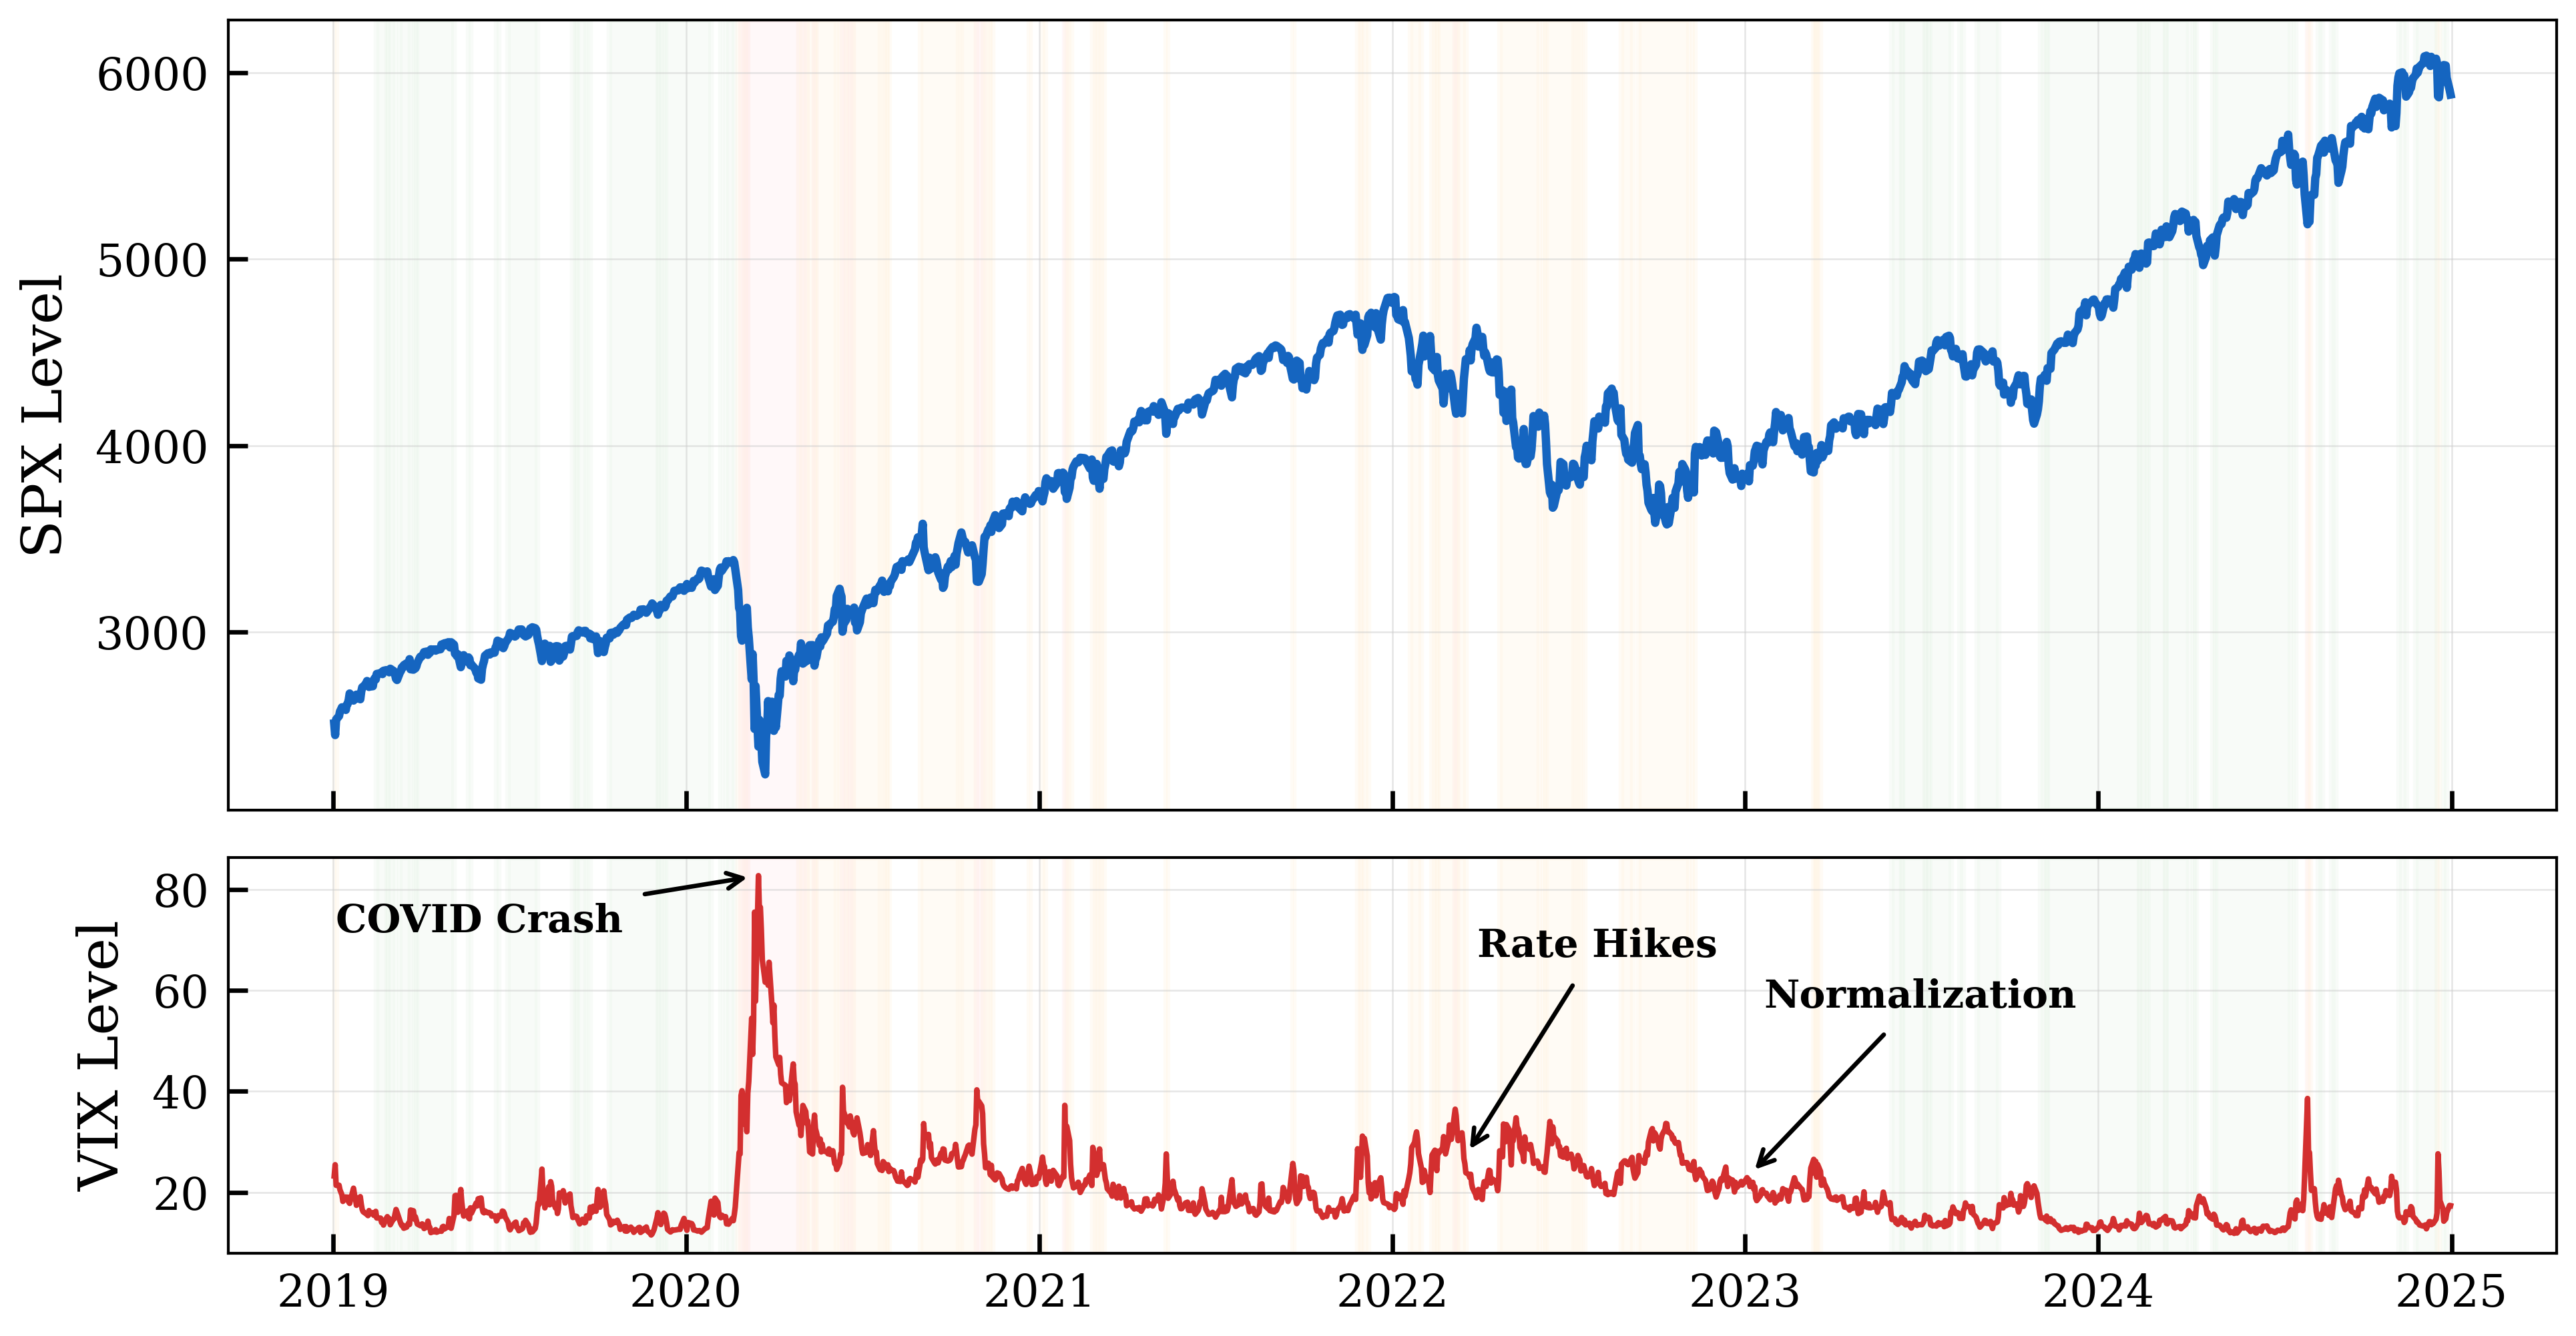
\includegraphics[width=\textwidth]{fig1_spx_vix.png}
\caption{SPX index level (top) and CBOE VIX (bottom) from January 2019 to December 2024. Background shading indicates VIX regime classification: Low (VIX $< 15$), Normal ($15$--$25$), High ($25$--$35$), and Crisis ($\geq 35$).}
\label{fig:spx_vix}
\end{figure}


% =============================================================================
% CHAPTER 5: EMPIRICAL RESULTS
% =============================================================================
\section{Empirical Results}
\label{sec:results}

\subsection{SVI Calibration Quality}
\label{sec:svi_quality}

I calibrate the Gatheral raw SVI parameterization on 3,131 (date, expiry) slices, of which 3,069 (98.0\%) converge to solutions with RMSE below the 300~bps threshold. Table~\ref{tab:svi_quality} summarizes calibration quality by VIX regime.

\begin{table}[H]
\centering
\caption{SVI calibration quality by VIX regime. Mean difference and RMSE are in basis points of implied volatility. $N$ is the number of option-day observations covered by each regime's calibrations.}
\label{tab:svi_quality}
\begin{tabular}{lrrrrrrr}
\toprule
Regime & $N$ & Mean Diff & Std Diff & MAE & RMSE & Median $|e|$ & $p_{95}|e|$ \\
\midrule
Low     & 8,457  & 23.1 & 127.4 & 83.4  & 129.5 & 47.6  & 311.4 \\
Normal  & 15,145 & 12.3 & 155.7 & 102.2 & 156.2 & 56.9  & 368.6 \\
High    & 10,442 & 4.3  & 168.4 & 109.8 & 168.4 & 59.9  & 387.5 \\
Crisis  & 8,982  & 6.7  & 179.2 & 105.1 & 179.4 & 17.1  & 425.8 \\
\midrule
ALL     & 43,026 & 11.3 & 159.2 & 100.9 & 159.6 & 48.0  & 380.9 \\
\bottomrule
\end{tabular}
\end{table}

The median calibration RMSE across all slices is 19.5 bps, with a mean of 38.6 bps and 95th percentile of 154.5 bps. These figures are consistent with the SVI calibration literature for liquid equity index options. Calibration quality degrades in high-volatility regimes, where smiles are steeper and less regular.

Figure~\ref{fig:svi_rmse} shows the time series of SVI calibration RMSE, and Figure~\ref{fig:svi_fit} provides examples of SVI fits across regimes.

\begin{figure}[H]
\centering
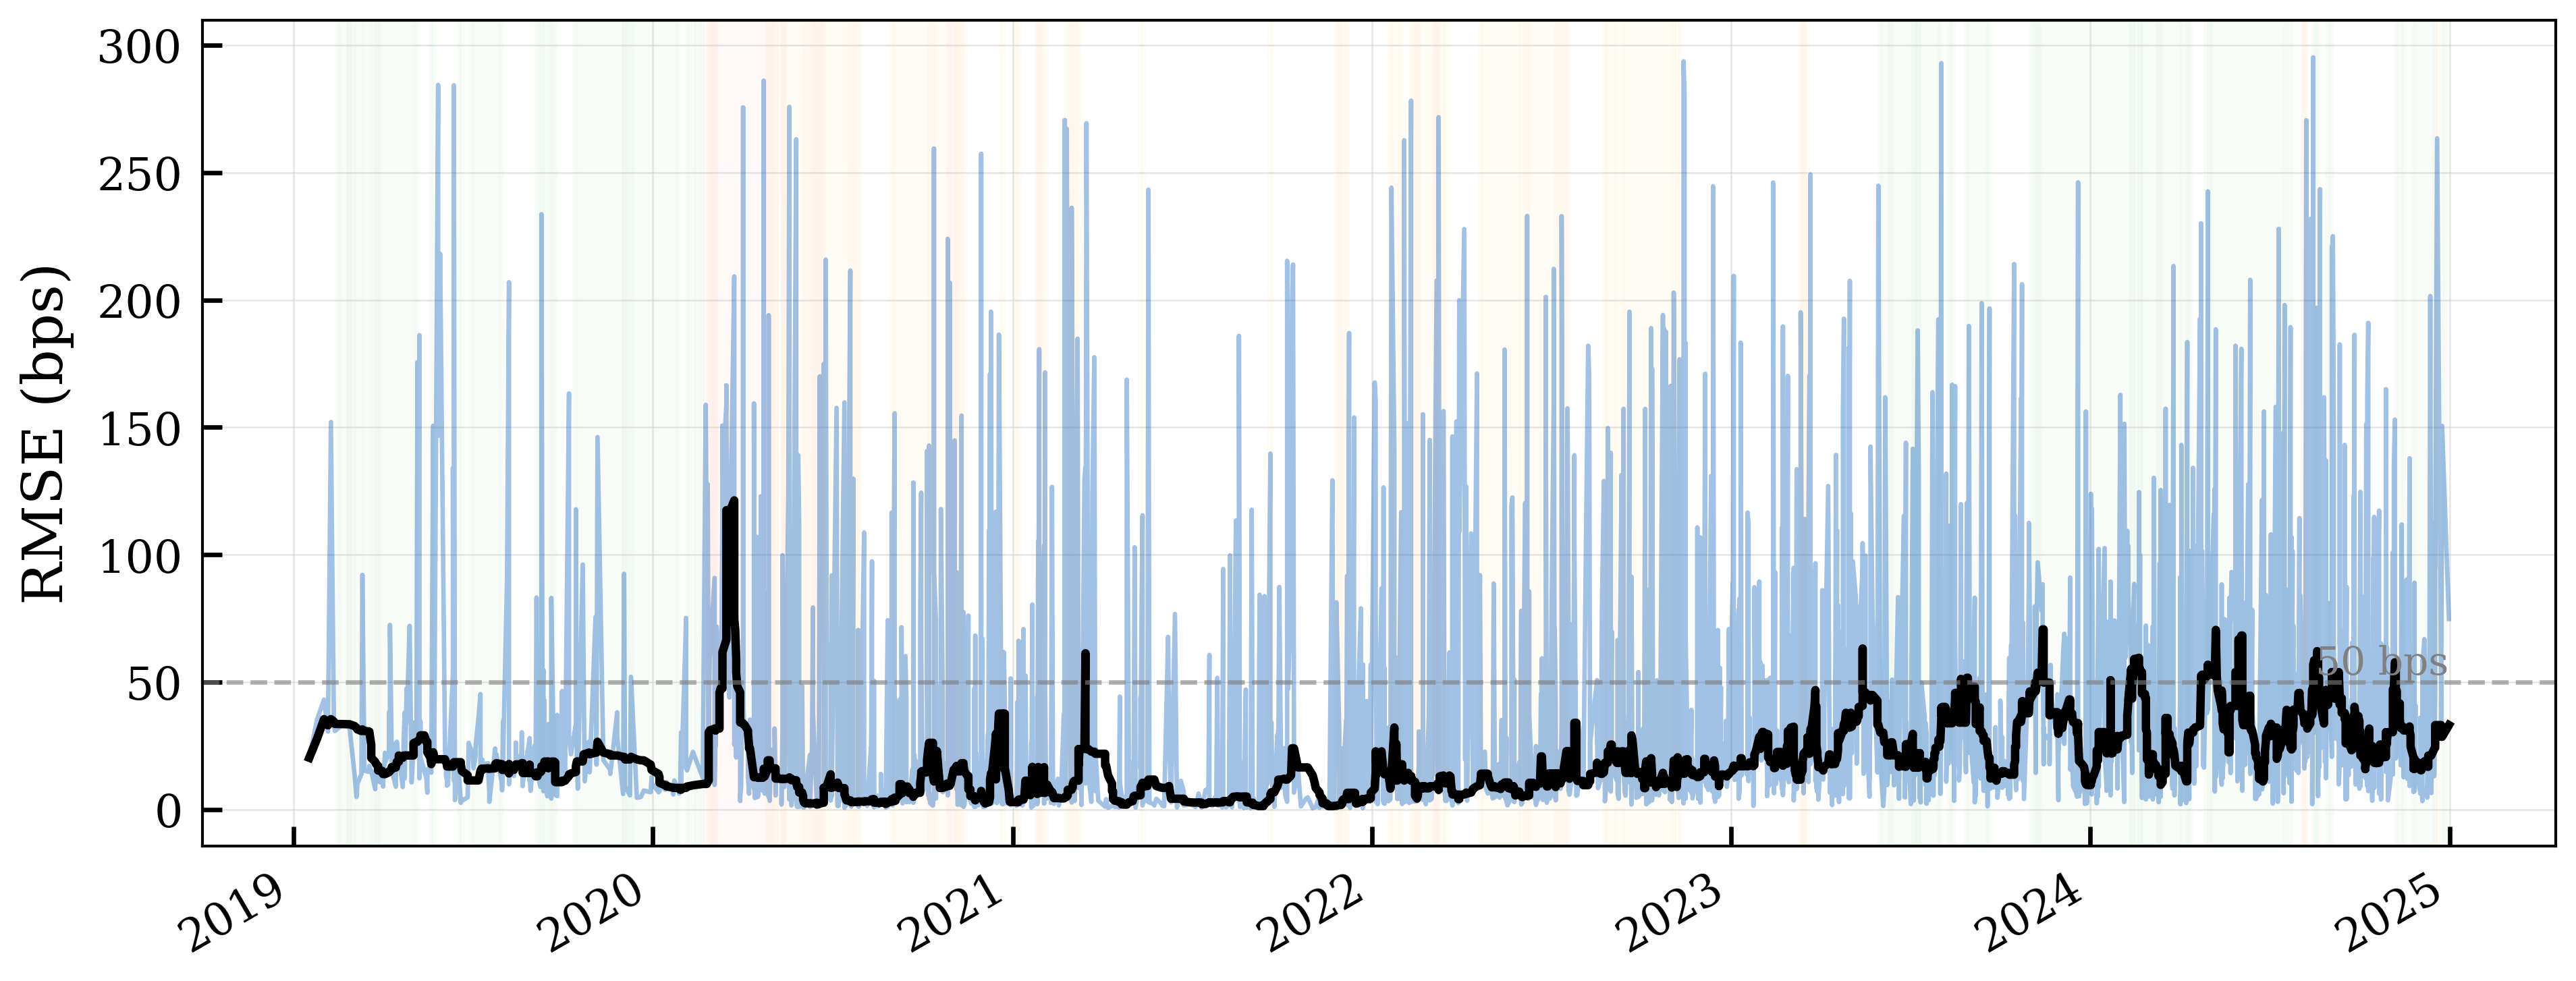
\includegraphics[width=\textwidth]{fig2_svi_rmse.png}
\caption{SVI calibration RMSE (bps) over time. Gray line shows daily values; black line shows 21-day moving average. Spikes coincide with high-VIX episodes where the smile is steep and irregular.}
\label{fig:svi_rmse}
\end{figure}

\begin{figure}[H]
\centering
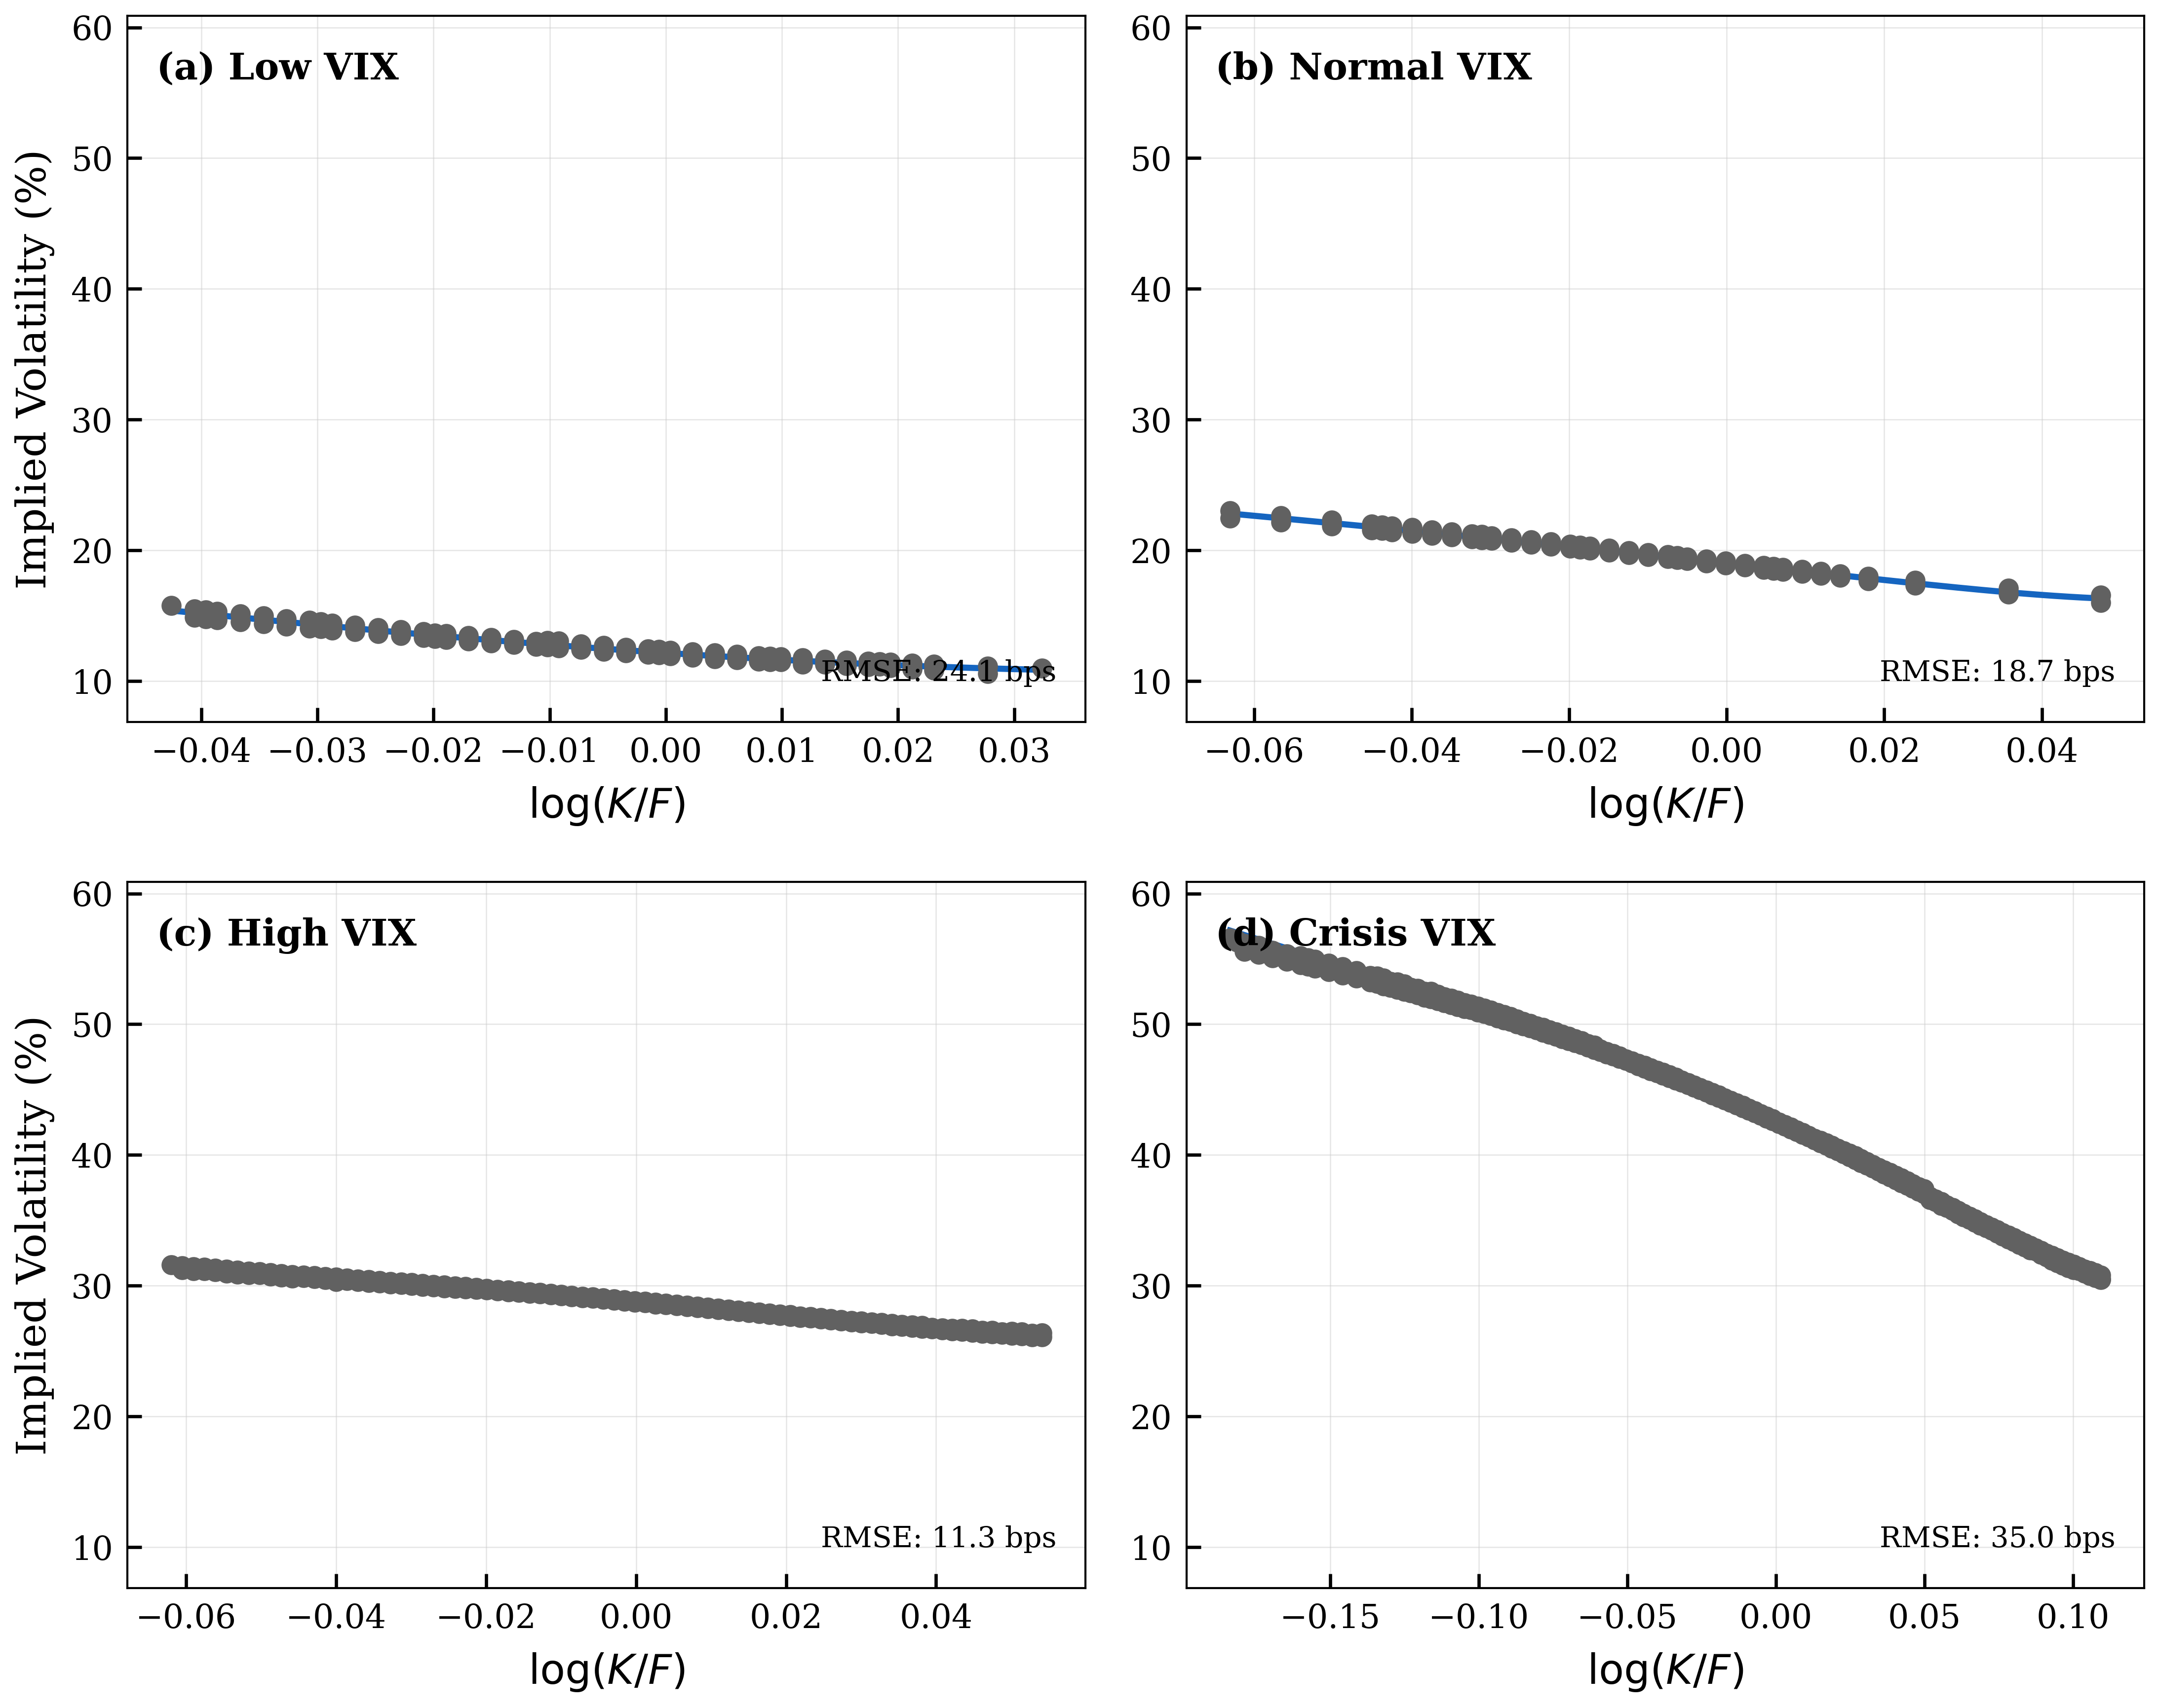
\includegraphics[width=\textwidth]{fig3_svi_fits.png}
\caption{Representative SVI calibration fits across VIX regimes. Each panel shows market implied volatilities (dots) versus the calibrated SVI curve (line) for a single (date, expiry) slice.}
\label{fig:svi_fit}
\end{figure}

\subsubsection{SVI Parameter Statistics}

Table~\ref{tab:svi_params} reports summary statistics for the five SVI parameters across all 3,069 successfully calibrated slices.

\begin{table}[H]
\centering
\caption{SVI parameter summary statistics across 3,069 calibrated slices. Brackets show the 5th--95th percentile range.}
\label{tab:svi_params}
\begin{tabular}{lccl}
\toprule
Parameter & Mean & Std & $[p_5, \, p_{95}]$ \\
\midrule
$a$      & $-0.0030$ & 0.0048 & $[-0.0112, +0.0031]$ \\
$b$      & $+0.0379$ & 0.0308 & $[+0.0064, +0.0930]$ \\
$\rho$   & $-0.3311$ & 0.3956 & $[-0.9895, +0.3603]$ \\
$m$      & $+0.0532$ & 0.1224 & $[-0.0496, +0.3955]$ \\
$\sigma$ & $+0.0971$ & 0.0854 & $[+0.0010, +0.2132]$ \\
\bottomrule
\end{tabular}
\end{table}

The negative mean $\rho$ confirms the well-documented negative skew of SPX implied volatility: puts are more expensive than calls. The wide range of $\rho$ (from $-0.99$ to $+0.36$) reflects variation in skew intensity across maturities and regimes.

\subsubsection{Butterfly Arbitrage Validation}

The Durrleman condition (Equation~\ref{eq:durrleman}) is satisfied on 2,105 of 3,069 calibrated slices (68.6\%). Table~\ref{tab:butterfly} reports the arbitrage-free rate by DTE bucket and RMSE bucket.

\begin{table}[H]
\centering
\caption{Butterfly arbitrage-free rates. Left panel: by days-to-expiry. Right panel: by calibration RMSE quality.}
\label{tab:butterfly}
\begin{minipage}{0.45\textwidth}
\centering
\begin{tabular}{lrr}
\toprule
DTE & Arb-Free & Rate \\
\midrule
0--30   & 1,538 / 2,359 & 65.2\% \\
31--60  & 491 / 616     & 79.7\% \\
61--90  & 76 / 94       & 80.9\% \\
\bottomrule
\end{tabular}
\end{minipage}
\hfill
\begin{minipage}{0.50\textwidth}
\centering
\begin{tabular}{lrr}
\toprule
RMSE (bps) & Arb-Free & Rate \\
\midrule
0--25       & 1,457 / 1,769 & 82.4\% \\
25--50      & 363 / 585     & 62.1\% \\
50--100     & 195 / 393     & 49.6\% \\
100--200    & 86 / 262      & 32.8\% \\
200--300    & 4 / 60        & 6.7\% \\
\bottomrule
\end{tabular}
\end{minipage}
\end{table}

Two patterns emerge. First, shorter-dated slices are harder to calibrate without arbitrage, likely because the smile is more curved and the total variance is smaller (making relative errors larger). Second, calibration quality strongly predicts arbitrage-free status: 82.4\% of slices with RMSE below 25 bps are arbitrage-free, compared to only 6.7\% of slices with RMSE above 200 bps. This suggests that enforcing arbitrage-free constraints---\eg, through SSVI \citep{Gatheral2014} or penalized optimization---would likely also improve calibration quality, and vice versa.

\subsection{Hedging Error Comparison: The Horse Race (H\ref{hyp:svi})}
\label{sec:horse_race}

Table~\ref{tab:hedging_main} presents the main hedging results across all 2,000 options and by VIX regime.

\begin{table}[H]
\centering
\caption{Hedging error comparison by volatility input and VIX regime. Std and RMSE are in dollars per option contract. Gain is the Hull \& White (2017) statistic: percentage reduction in hedging error std relative to Flat BSM.}
\label{tab:hedging_main}
\small
\begin{tabular}{llrrrrrrr}
\toprule
Vol Input & Regime & $N$ & Mean & Std & MAE & RMSE & Gain (\%) & \% Pos \\
\midrule
Flat BSM        & ALL     & 2,000 & 3.60  & 42.10 & 31.12 & 42.24 & 0.0    & 70.9 \\
SVI Surface     & ALL     & 2,000 & $-0.31$ & 46.04 & 32.64 & 46.03 & $-9.4$  & 69.5 \\
RV (CC)         & ALL     & 2,000 & 6.39  & 39.66 & 29.43 & 40.17 & $+5.8$  & 66.1 \\
RV (Parkinson)  & ALL     & 2,000 & $-17.95$ & 60.30 & 38.41 & 62.90 & $-43.2$ & 54.0 \\
RV (Yang--Zhang) & ALL    & 2,000 & $-5.08$ & 49.86 & 34.19 & 50.11 & $-18.4$ & 61.7 \\
\midrule
Flat BSM        & Low     & 500 & 8.10  & 18.36 & 15.99 & 20.05 & 0.0    & 71.8 \\
SVI Surface     & Low     & 500 & 7.45  & 19.98 & 16.68 & 21.30 & $-8.8$  & 69.2 \\
RV (CC)         & Low     & 500 & 4.68  & 19.66 & 15.66 & 20.19 & $-7.1$  & 64.2 \\
\midrule
Flat BSM        & Normal  & 500 & 19.71 & 18.20 & 22.60 & 26.81 & 0.0    & 87.6 \\
SVI Surface     & Normal  & 500 & 19.21 & 18.05 & 22.00 & 26.35 & $+0.8$  & 86.6 \\
RV (CC)         & Normal  & 500 & 12.73 & 20.98 & 19.81 & 24.52 & $-15.3$ & 79.2 \\
\midrule
Flat BSM        & High    & 500 & 19.37 & 20.64 & 24.48 & 28.28 & 0.0    & 83.6 \\
SVI Surface     & High    & 500 & 19.28 & 19.87 & 23.76 & 27.67 & $+3.7$  & 82.4 \\
RV (CC)         & High    & 500 & 18.19 & 23.19 & 25.36 & 29.45 & $-12.4$ & 77.8 \\
\midrule
Flat BSM        & Crisis  & 500 & $-32.79$ & 64.42 & 61.40 & 72.23 & 0.0    & 40.4 \\
SVI Surface     & Crisis  & 500 & $-47.18$ & 65.91 & 68.12 & 81.00 & $-2.3$  & 39.6 \\
RV (CC)         & Crisis  & 500 & $-10.05$ & 66.97 & 56.87 & 67.65 & $-4.0$  & 43.0 \\
\bottomrule
\end{tabular}
\end{table}

The aggregate results are clear: \textbf{Hypothesis~\ref{hyp:svi} is rejected.} SVI surface IV does not reduce hedging error variance relative to flat BSM IV. In fact, SVI produces a Gain of $-9.4\%$, meaning hedging error standard deviation \textit{increases} by 9.4\% when using SVI-calibrated volatilities instead of flat ATM IV. This increase is statistically significant (Table~\ref{tab:stat_tests}).

The only volatility input that outperforms the flat BSM benchmark in aggregate is close-to-close realized volatility, with a Gain of $+5.8\%$ and a statistically significant reduction in both variance ($F = 0.89$, $p = 0.008$) and mean absolute error ($t = -4.51$, $p < 0.001$).

Figure~\ref{fig:hedge_dist} shows the hedging error distributions, and Figure~\ref{fig:hedge_regime} shows hedging error standard deviation by regime.

\begin{figure}[H]
\centering
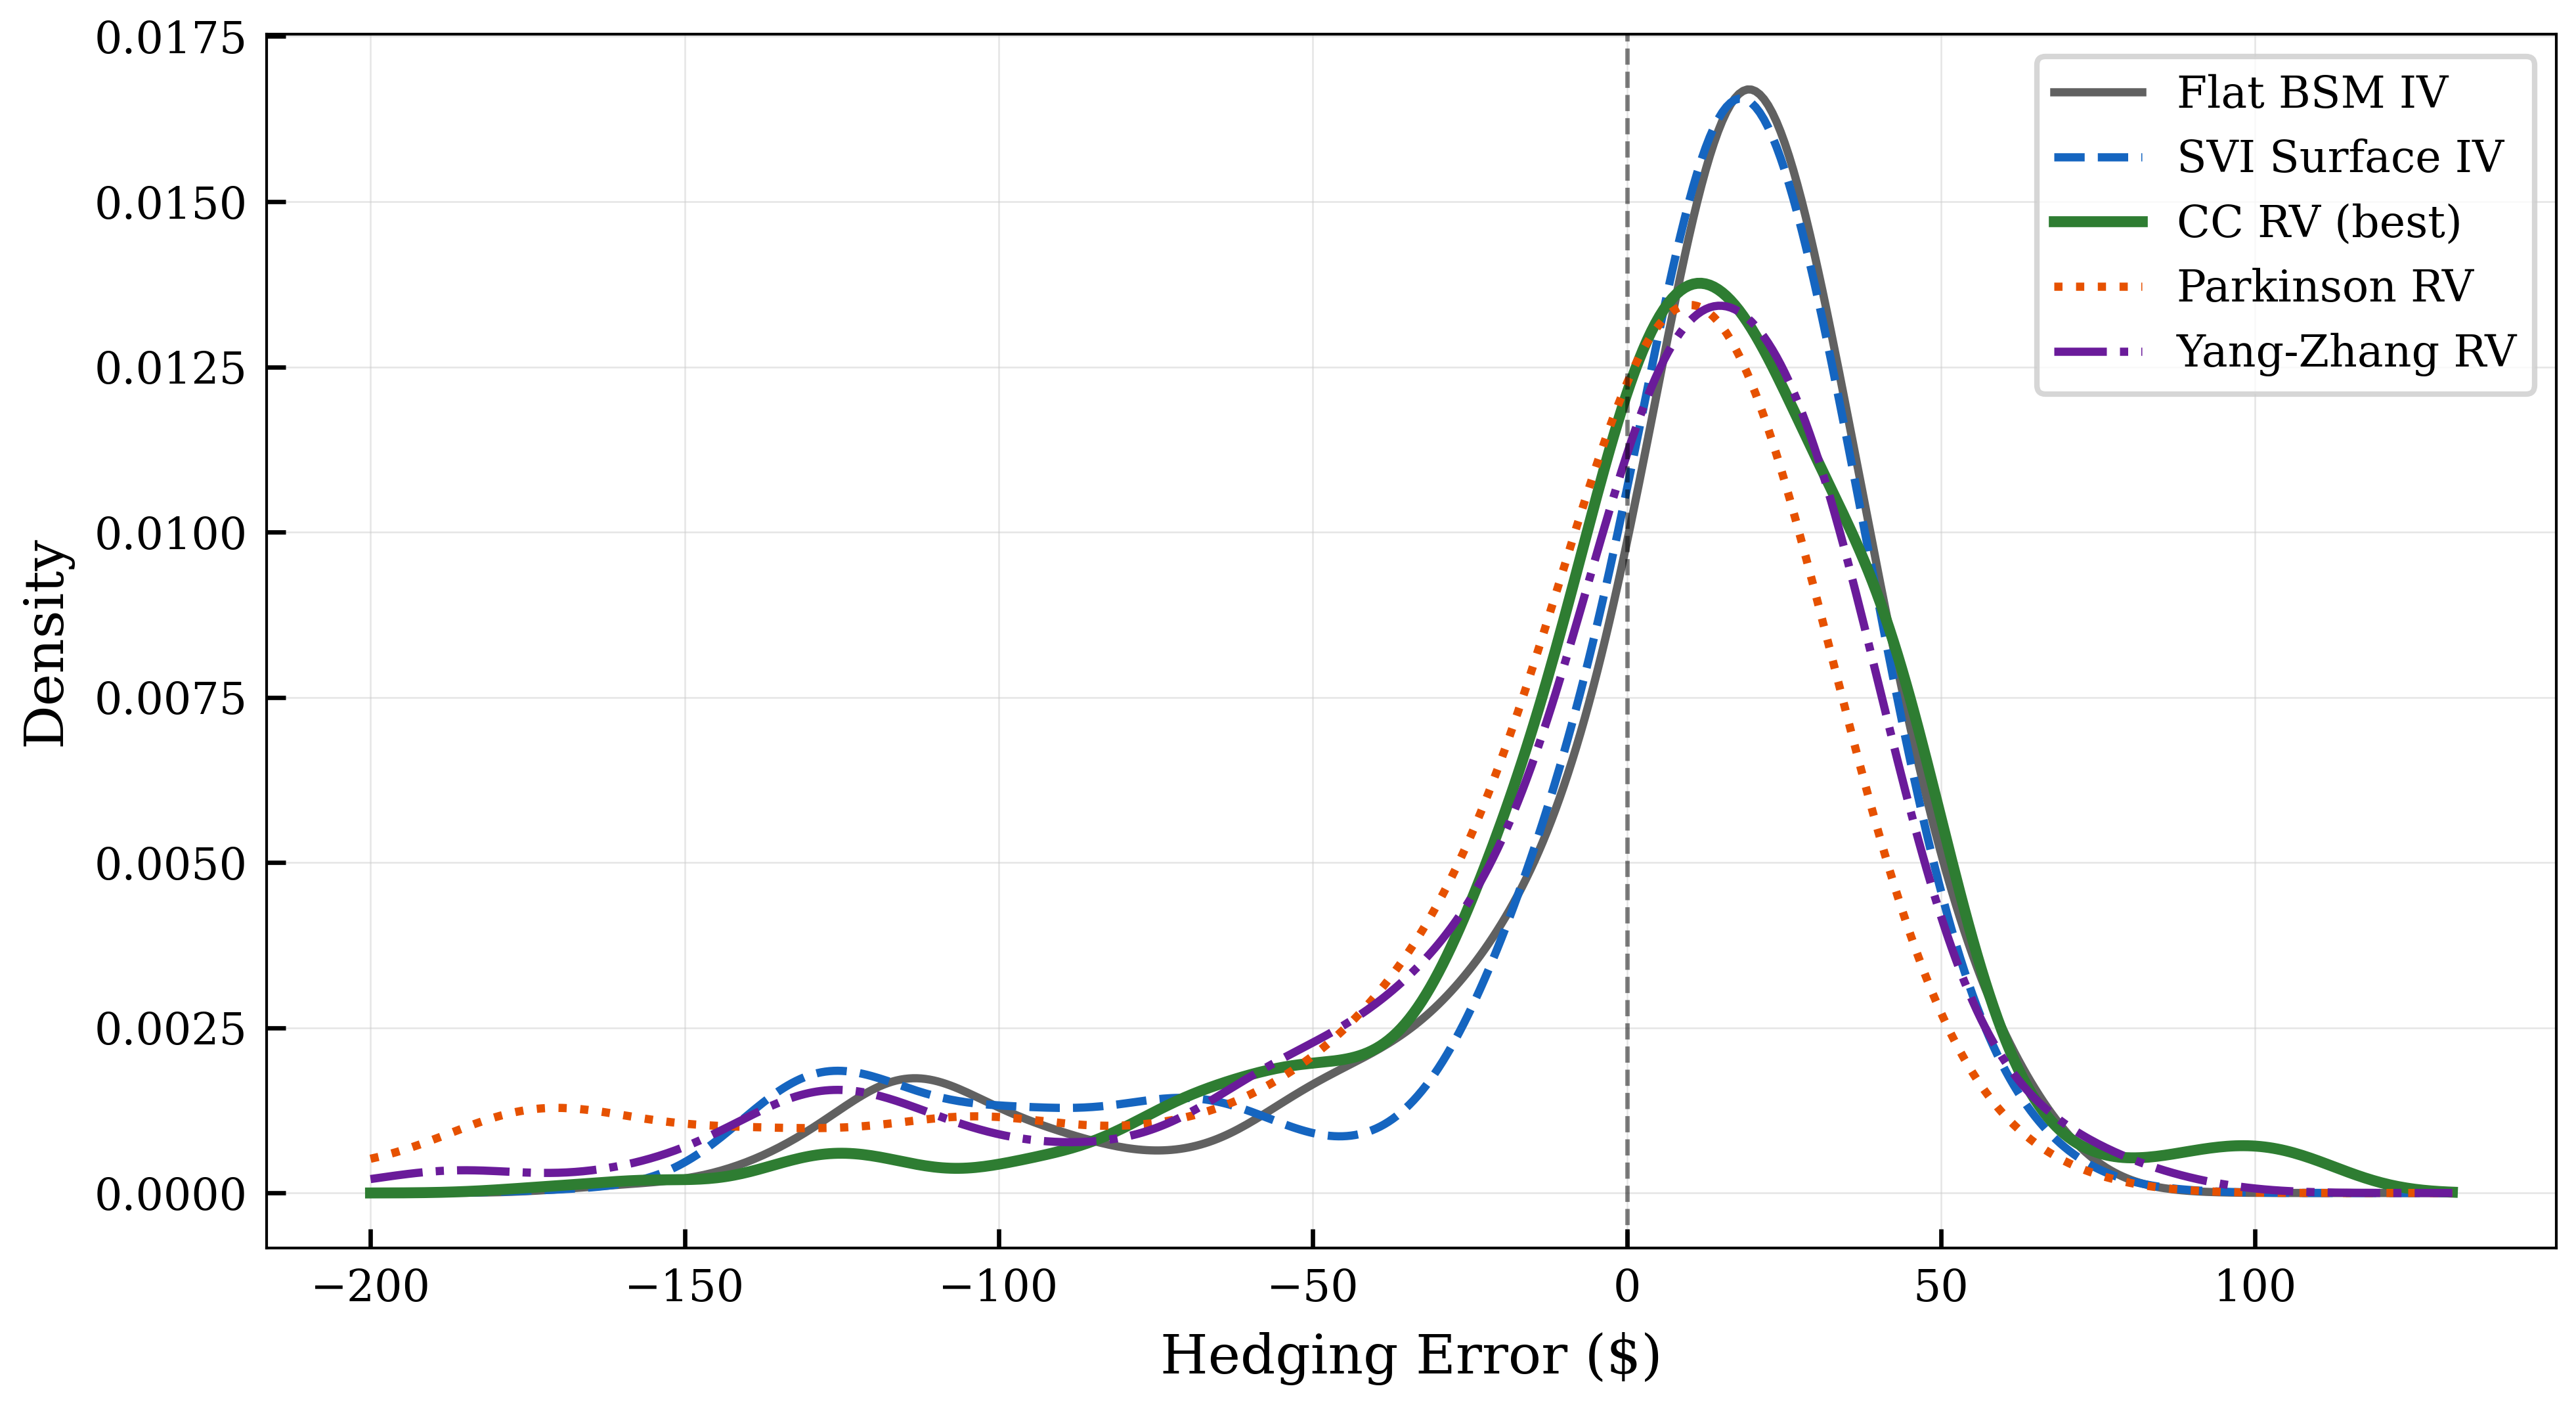
\includegraphics[width=\textwidth]{fig4_hedging_kde.png}
\caption{Hedging error distributions for the five volatility inputs. The vertical dashed line at zero represents perfect hedging.}
\label{fig:hedge_dist}
\end{figure}

\begin{figure}[H]
\centering
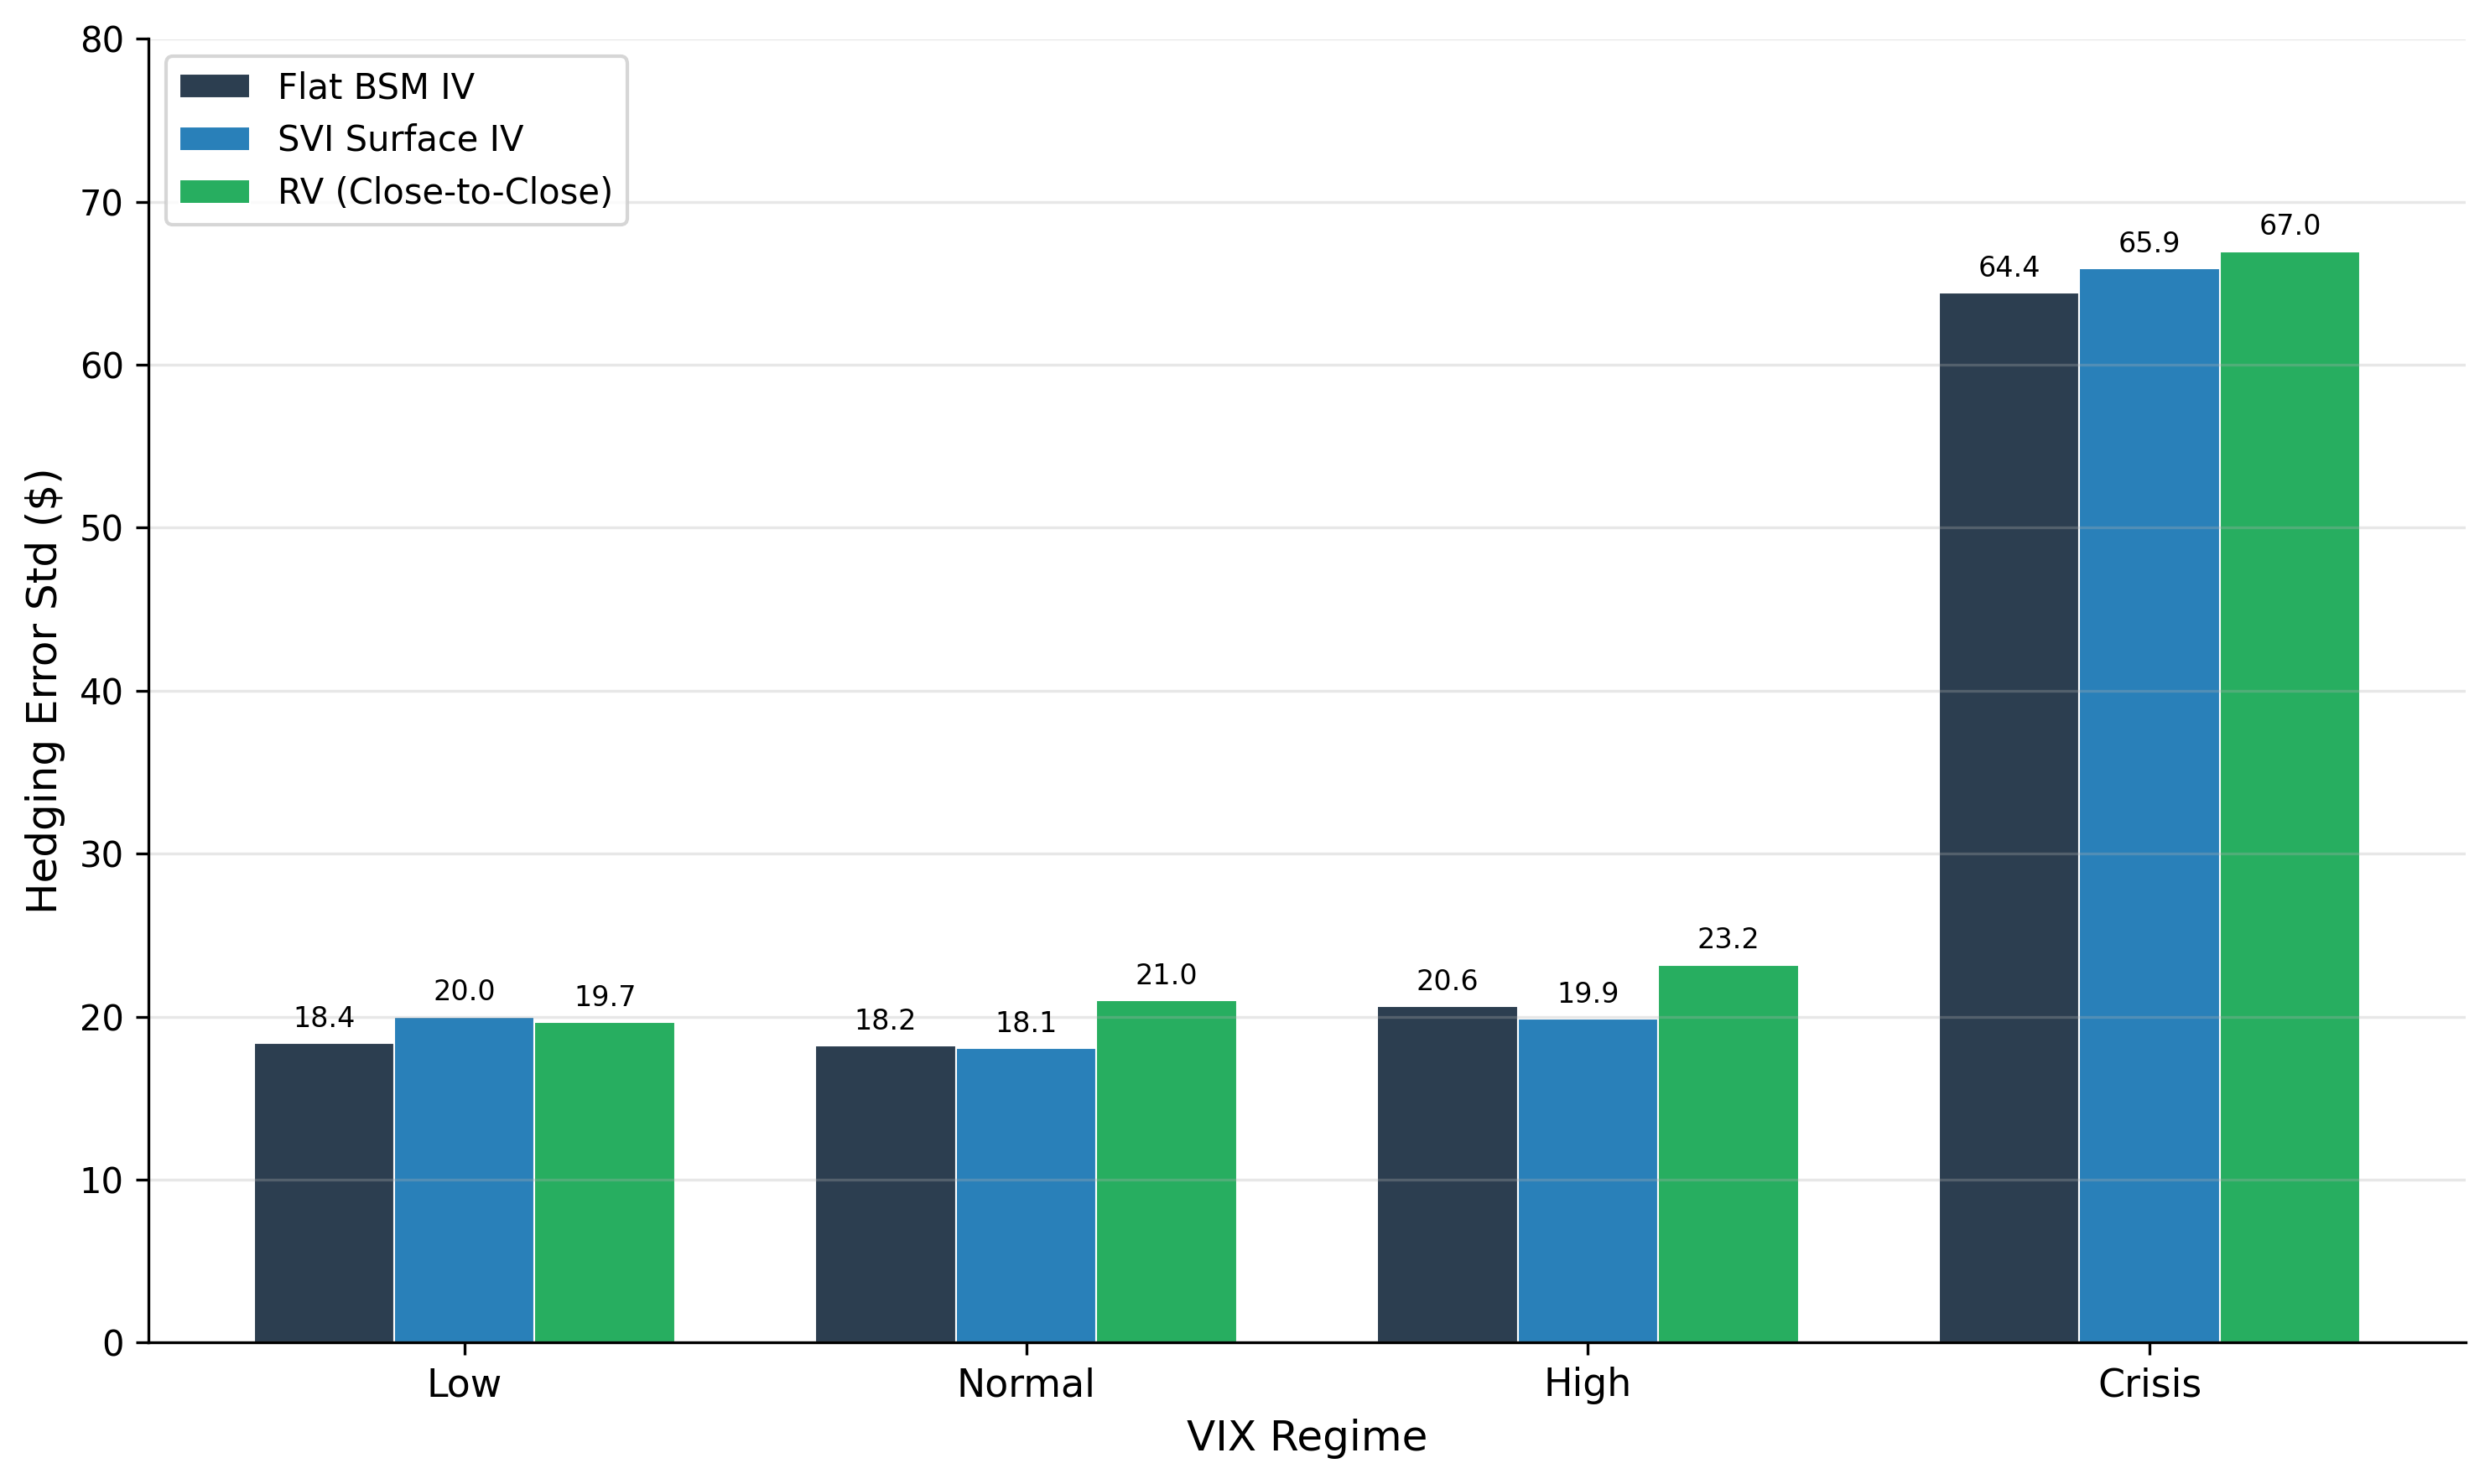
\includegraphics[width=\textwidth]{fig5_hedging_by_regime.png}
\caption{Hedging error standard deviation by VIX regime for each volatility input. Lower bars indicate better hedging performance.}
\label{fig:hedge_regime}
\end{figure}

\subsection{Realized Volatility Estimator Comparison (H\ref{hyp:yz})}
\label{sec:rv_comparison}

\textbf{Hypothesis~\ref{hyp:yz} is also rejected.} Yang--Zhang does not outperform close-to-close as a hedging input. In fact, close-to-close is the best-performing realized volatility estimator and the best overall volatility input:

\begin{center}
\begin{tabular}{lrr}
\toprule
RV Estimator & Std & Gain (\%) \\
\midrule
Close-to-Close & 39.66 & $+5.8$ \\
Yang--Zhang    & 49.86 & $-18.4$ \\
Parkinson      & 60.30 & $-43.2$ \\
\bottomrule
\end{tabular}
\end{center}

This ordering reverses the statistical efficiency ranking of these estimators. Parkinson, the most efficient under GBM assumptions, produces the worst hedging. The explanation is that ``more efficient'' in the statistical sense means these estimators are more sensitive to intraday price movements, which introduces noise in the hedging volatility. The close-to-close estimator's simplicity---using only closing prices---appears to be a feature, not a bug, for hedging purposes: it smooths out intraday noise that does not correspond to the close-to-close returns that drive option repricing.

Figure~\ref{fig:rv_iv} shows the time series of the three realized volatility estimators alongside the 30-day ATM implied volatility, illustrating how they diverge during high-volatility episodes.

\begin{figure}[H]
\centering
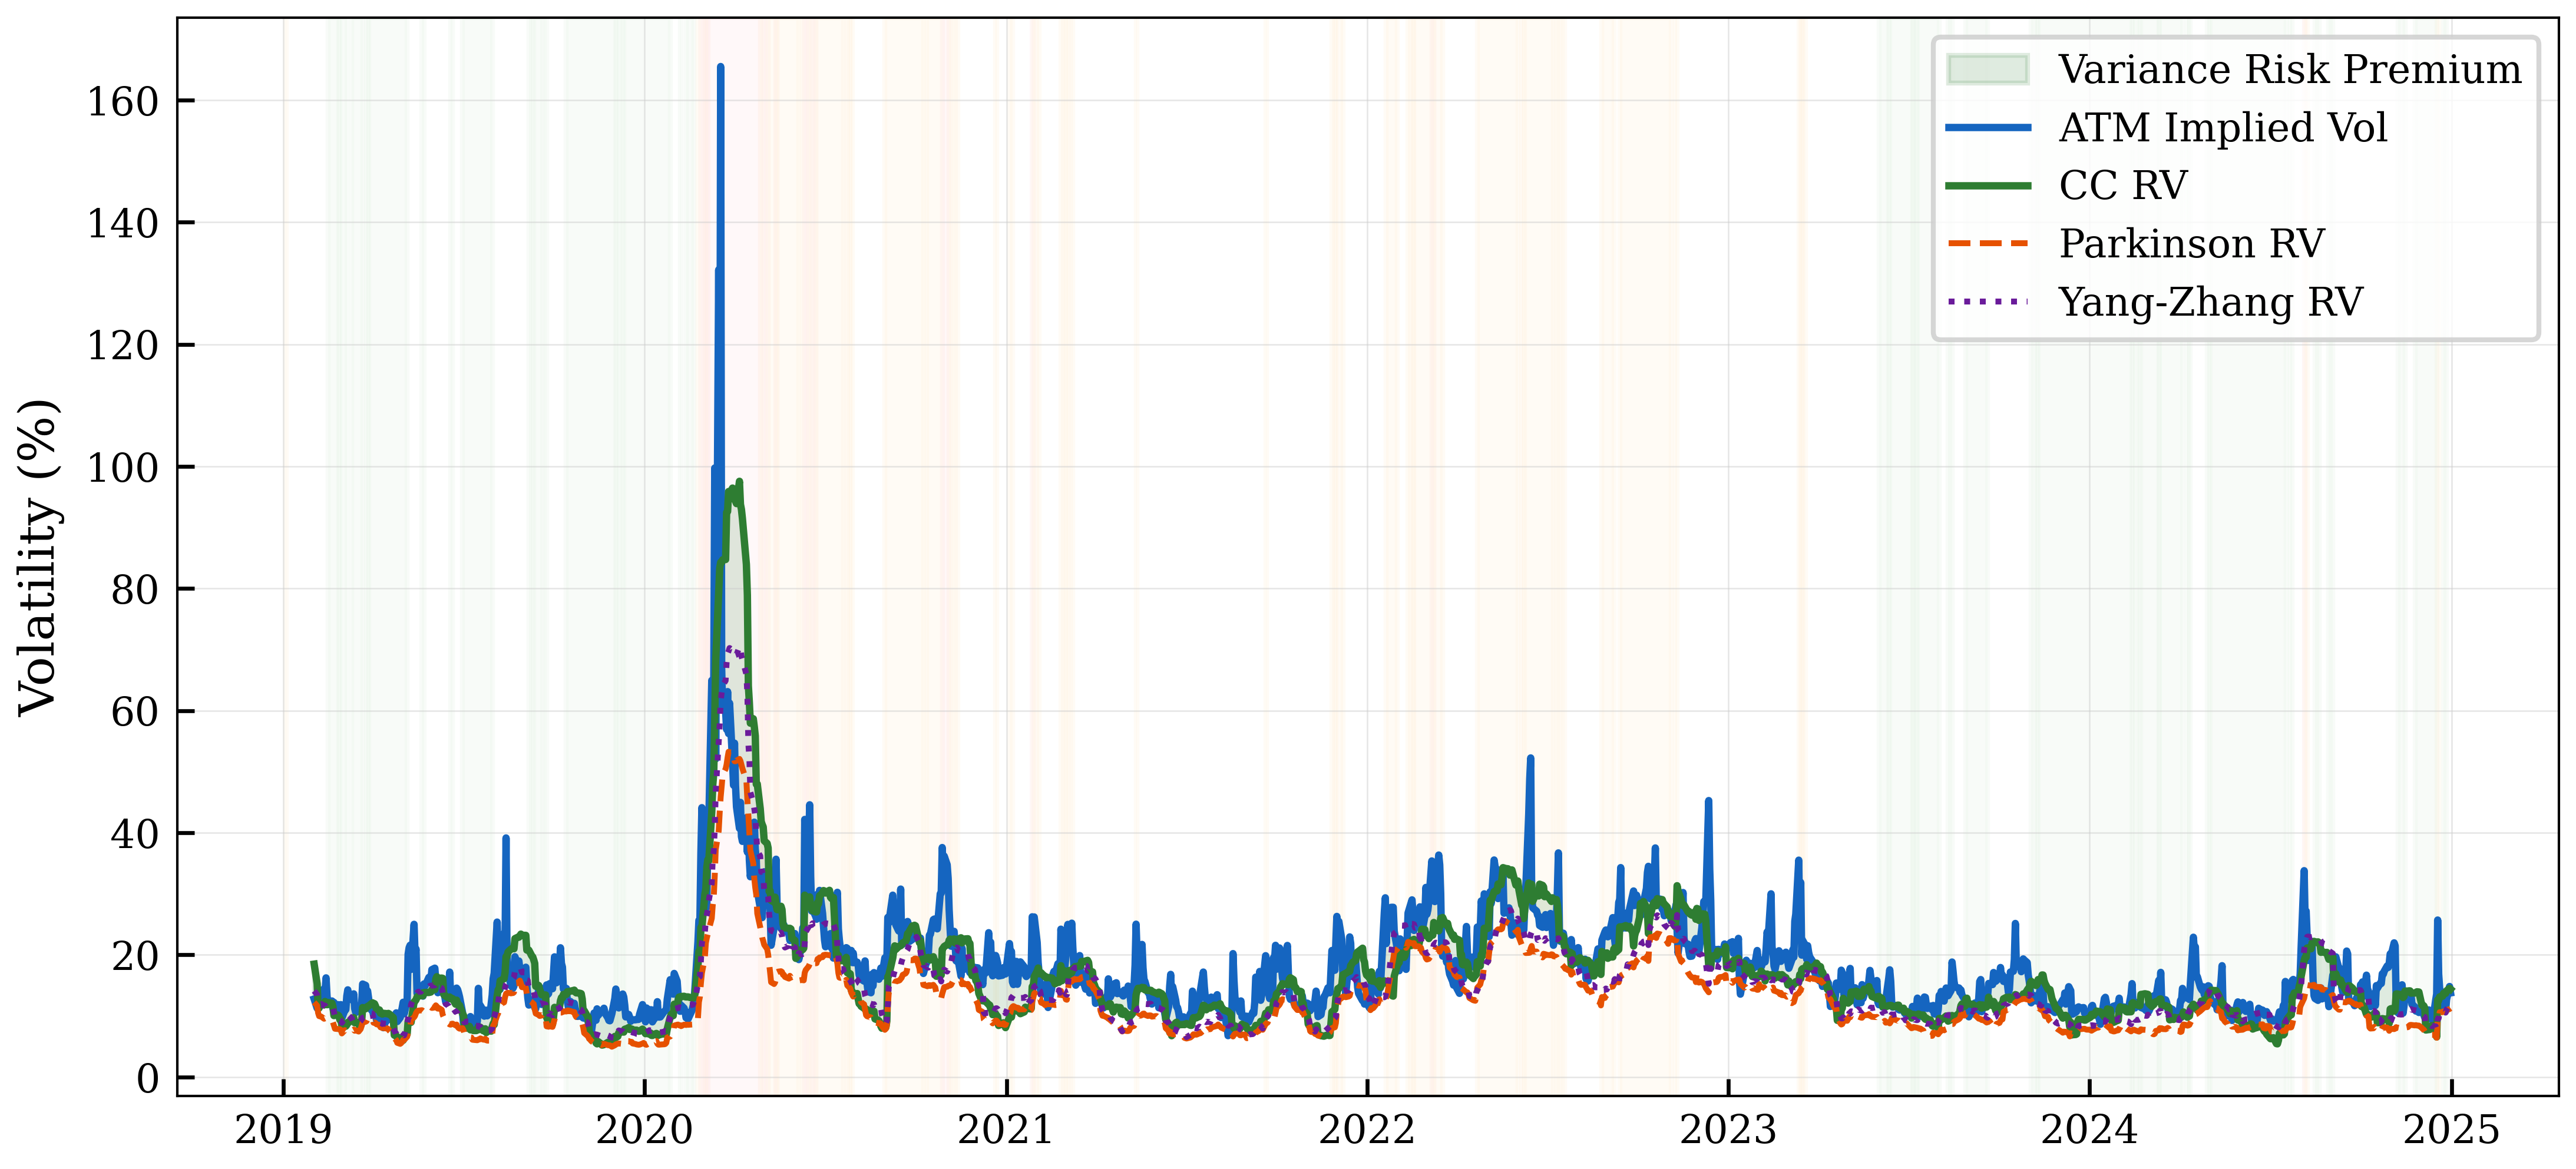
\includegraphics[width=\textwidth]{fig7_rv_vs_iv.png}
\caption{Realized volatility estimators (21-day rolling) and 30-day ATM implied volatility over the sample period. The Parkinson and Yang--Zhang estimators exhibit greater responsiveness to intraday volatility spikes.}
\label{fig:rv_iv}
\end{figure}

\subsection{Regime-Conditional Analysis (H\ref{hyp:regime})}
\label{sec:regime_analysis}

\textbf{Hypothesis~\ref{hyp:regime} receives partial support.} The optimal volatility input does vary by regime, though not in the way hypothesized:

\begin{itemize}
    \item \textbf{Low VIX:} Flat BSM wins (std = 18.36). All alternatives add noise.
    \item \textbf{Normal VIX:} SVI shows its only positive aggregate Gain ($+0.8\%$, std = 18.05 vs.\ 18.20). The smile provides marginal benefit when markets are orderly.
    \item \textbf{High VIX:} SVI shows its strongest Gain ($+3.7\%$, std = 19.87 vs.\ 20.64). The smile is steep enough to matter, and calibration quality is still acceptable.
    \item \textbf{Crisis:} Everything struggles. RV (CC) has the smallest degradation (Gain = $-4.0\%$), but all methods produce large errors (std $> 64$).
\end{itemize}

The more interesting regime dependence emerges at the moneyness level. Table~\ref{tab:best_vol} shows the best-performing volatility input for each moneyness$\times$maturity cell.

\begin{table}[H]
\centering
\caption{Best volatility input by moneyness and maturity. RMSE is in dollars per option. Bold indicates the winning method for each cell.}
\label{tab:best_vol}
\small
\begin{tabular}{llrrrrrrl}
\toprule
Moneyness & Mat. & $N$ & \multicolumn{5}{c}{RMSE by Vol Input} & Best \\
\cmidrule(lr){4-8}
          &      &     & Flat & SVI & CC & Park & YZ & \\
\midrule
ATM            & Short  & 292 & \textbf{24.4} & 24.6 & 26.2 & 26.3 & 25.7 & Flat BSM \\
ATM            & Medium & 167 & 27.4 & 28.1 & 25.4 & 25.6 & \textbf{24.0} & YZ \\
ATM            & Long   & 27  & 24.4 & 27.4 & 23.7 & 24.1 & \textbf{23.4} & YZ \\
Deep OTM Call  & Short  & 56  & 40.9 & \textbf{36.1} & 69.5 & 49.4 & 56.8 & SVI \\
Deep OTM Call  & Medium & 56  & 46.1 & 24.0 & 76.0 & \textbf{16.8} & 47.2 & Park \\
Deep OTM Put   & Short  & 81  & \textbf{93.9} & 99.2 & 96.6 & 175.9 & 138.4 & Flat BSM \\
Deep OTM Put   & Medium & 119 & 90.1 & 108.4 & \textbf{58.6} & 153.8 & 109.7 & CC \\
Deep OTM Put   & Long   & 21  & 101.3 & 114.1 & \textbf{53.3} & 136.7 & 95.2 & CC \\
OTM Call       & Short  & 455 & 24.5 & \textbf{23.0} & 27.1 & 30.1 & 26.7 & SVI \\
OTM Call       & Medium & 261 & 28.8 & \textbf{25.6} & 28.0 & 26.2 & 25.9 & SVI \\
OTM Call       & Long   & 48  & 37.5 & 37.2 & 31.4 & 33.7 & \textbf{29.8} & YZ \\
OTM Put        & Short  & 194 & \textbf{42.3} & 43.4 & 43.0 & 49.2 & 45.7 & Flat BSM \\
OTM Put        & Medium & 187 & 32.4 & 47.5 & \textbf{25.5} & 53.4 & 36.6 & CC \\
OTM Put        & Long   & 33  & 33.0 & 43.0 & \textbf{23.0} & 47.2 & 34.4 & CC \\
\bottomrule
\end{tabular}
\end{table}

The pattern is striking:
\begin{itemize}
    \item \textbf{SVI dominates for OTM calls} (short and medium maturity), with RMSE reductions of 6--12\% versus flat BSM. This is the segment where the volatility smile has the steepest slope, so strike-specific IV provides the most informational value.
    \item \textbf{RV (CC) dominates for OTM puts} (medium and long maturity), with RMSE reductions of 21--48\%. OTM puts have embedded skew premium that makes implied-based methods systematically biased.
    \item \textbf{Flat BSM wins for ATM short-dated} and \textbf{RV (YZ) wins for ATM medium/long-dated} options.
    \item \textbf{No single input wins everywhere.}
\end{itemize}

These results strongly support the view that the optimal hedging volatility is both regime- and moneyness-dependent.

\subsection{P\&L Attribution by Regime}
\label{sec:pnl_attribution}

Table~\ref{tab:pnl_attrib} reports the covariance-based variance attribution (Equation~\ref{eq:cov_decomp}) for the flat BSM benchmark across VIX regimes.

\begin{table}[H]
\centering
\caption{P\&L variance attribution for Flat BSM hedging by VIX regime. Contributions are percentages of total hedging error variance, computed via covariance decomposition (Equation~\ref{eq:cov_decomp}). Contributions sum to 100\% within each regime.}
\label{tab:pnl_attrib}
\begin{tabular}{lrrrr}
\toprule
Regime & $N$ & Discrete (\%) & Vol Misspec (\%) & Residual (\%) \\
\midrule
Low     & 500 & $-38.4$ & $-20.0$ & 158.4 \\
Normal  & 500 & $-51.4$ & $-10.1$ & 161.5 \\
High    & 500 & $-58.8$ & 6.0     & 152.8 \\
Crisis  & 500 & $-57.7$ & $-4.2$  & 161.9 \\
\midrule
ALL     & 2,000 & $-70.8$ & $-72.1$ & 242.9 \\
\bottomrule
\end{tabular}
\end{table}

The negative covariance contributions for discrete rebalancing error indicate that this component is negatively correlated with total P\&L: when discrete rebalancing produces a gain, the total tends to be a loss, and vice versa. This reflects the well-known gamma--theta offset---discrete rebalancing error is partially offset by the theta component embedded in the option's market price changes. The large positive residual contribution (153--162\%) dominates across all regimes, indicating that higher-order effects (vanna, volga, jumps, and model misspecification beyond volatility) are the primary drivers of hedging P\&L variance.

Figure~\ref{fig:pnl_attrib} visualizes the attribution across all five volatility inputs and four regimes.

\begin{figure}[H]
\centering
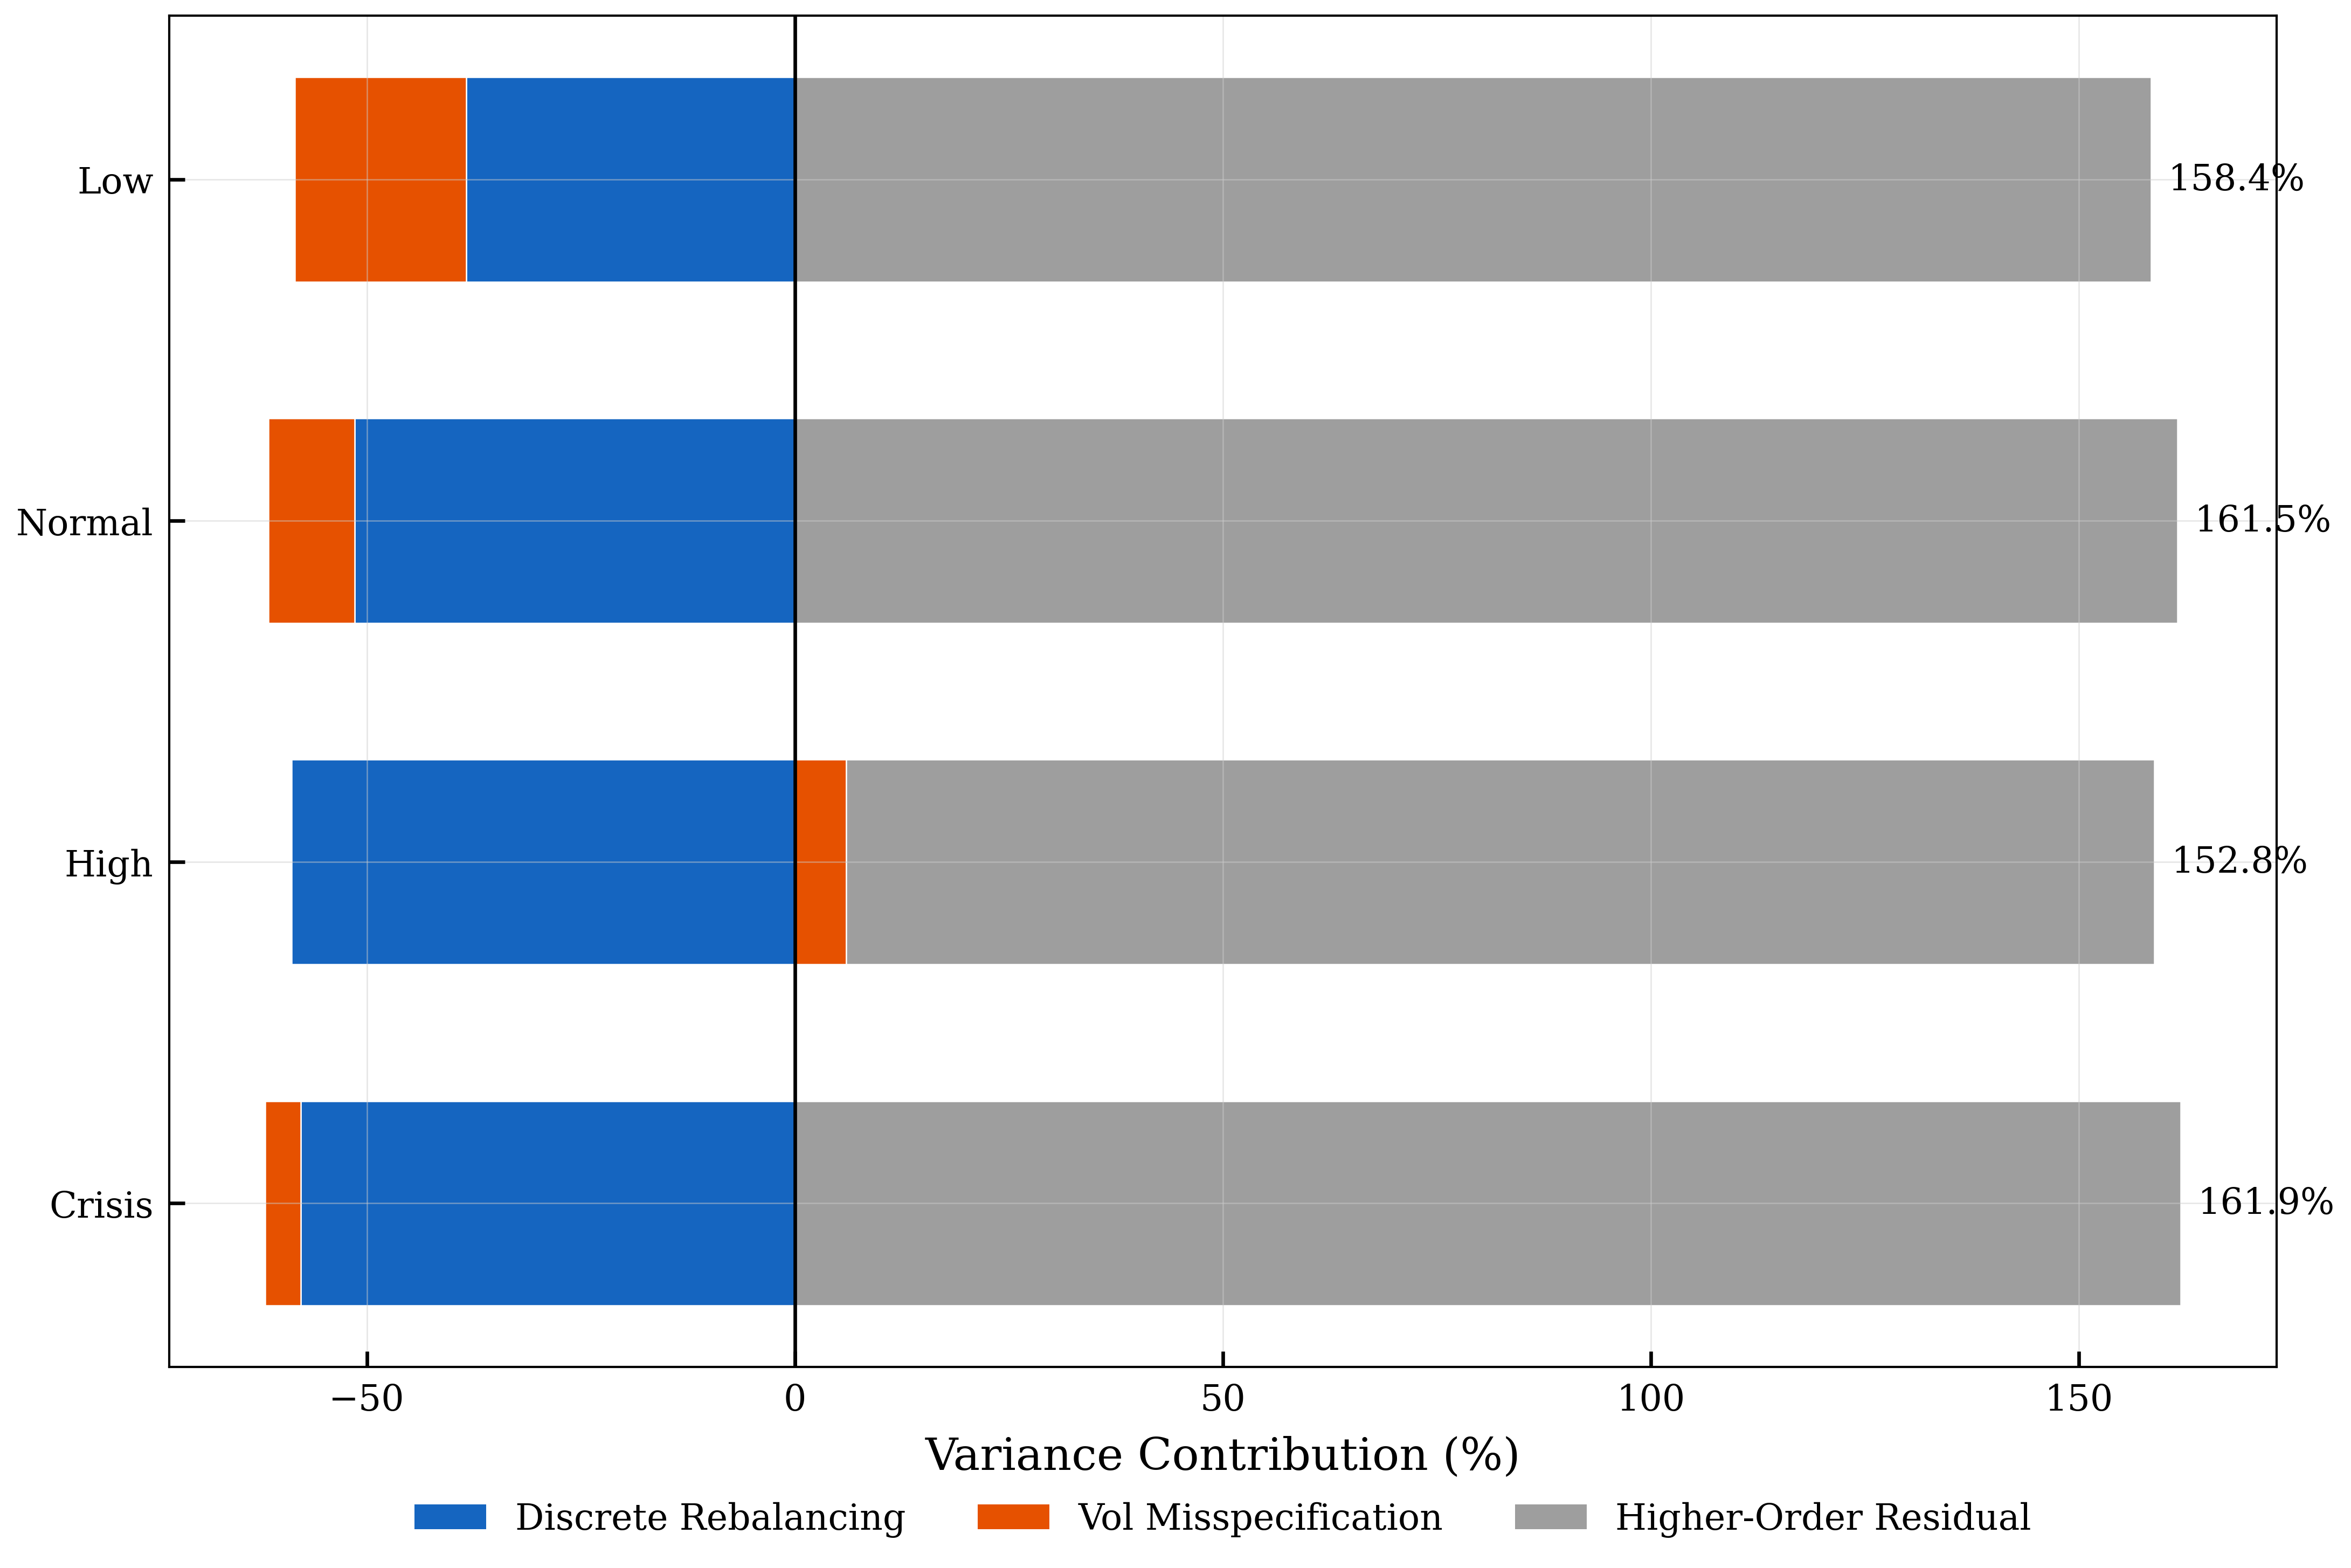
\includegraphics[width=\textwidth]{fig6_pnl_attribution.png}
\caption{P\&L variance attribution by VIX regime and volatility input. Each stacked bar decomposes total hedging error variance into discrete rebalancing error, volatility misspecification, and higher-order residual components. Contributions are computed via covariance decomposition and sum to 100\%.}
\label{fig:pnl_attrib}
\end{figure}

\subsection{SVI Calibration Quality as a Hedging Predictor}
\label{sec:svi_predictor}

If SVI calibration quality drives hedging performance, one should observe a positive relationship between calibration RMSE and absolute hedging error. Figure~\ref{fig:svi_hedge} tests this hypothesis via a scatter plot with OLS regression.

\begin{figure}[H]
\centering
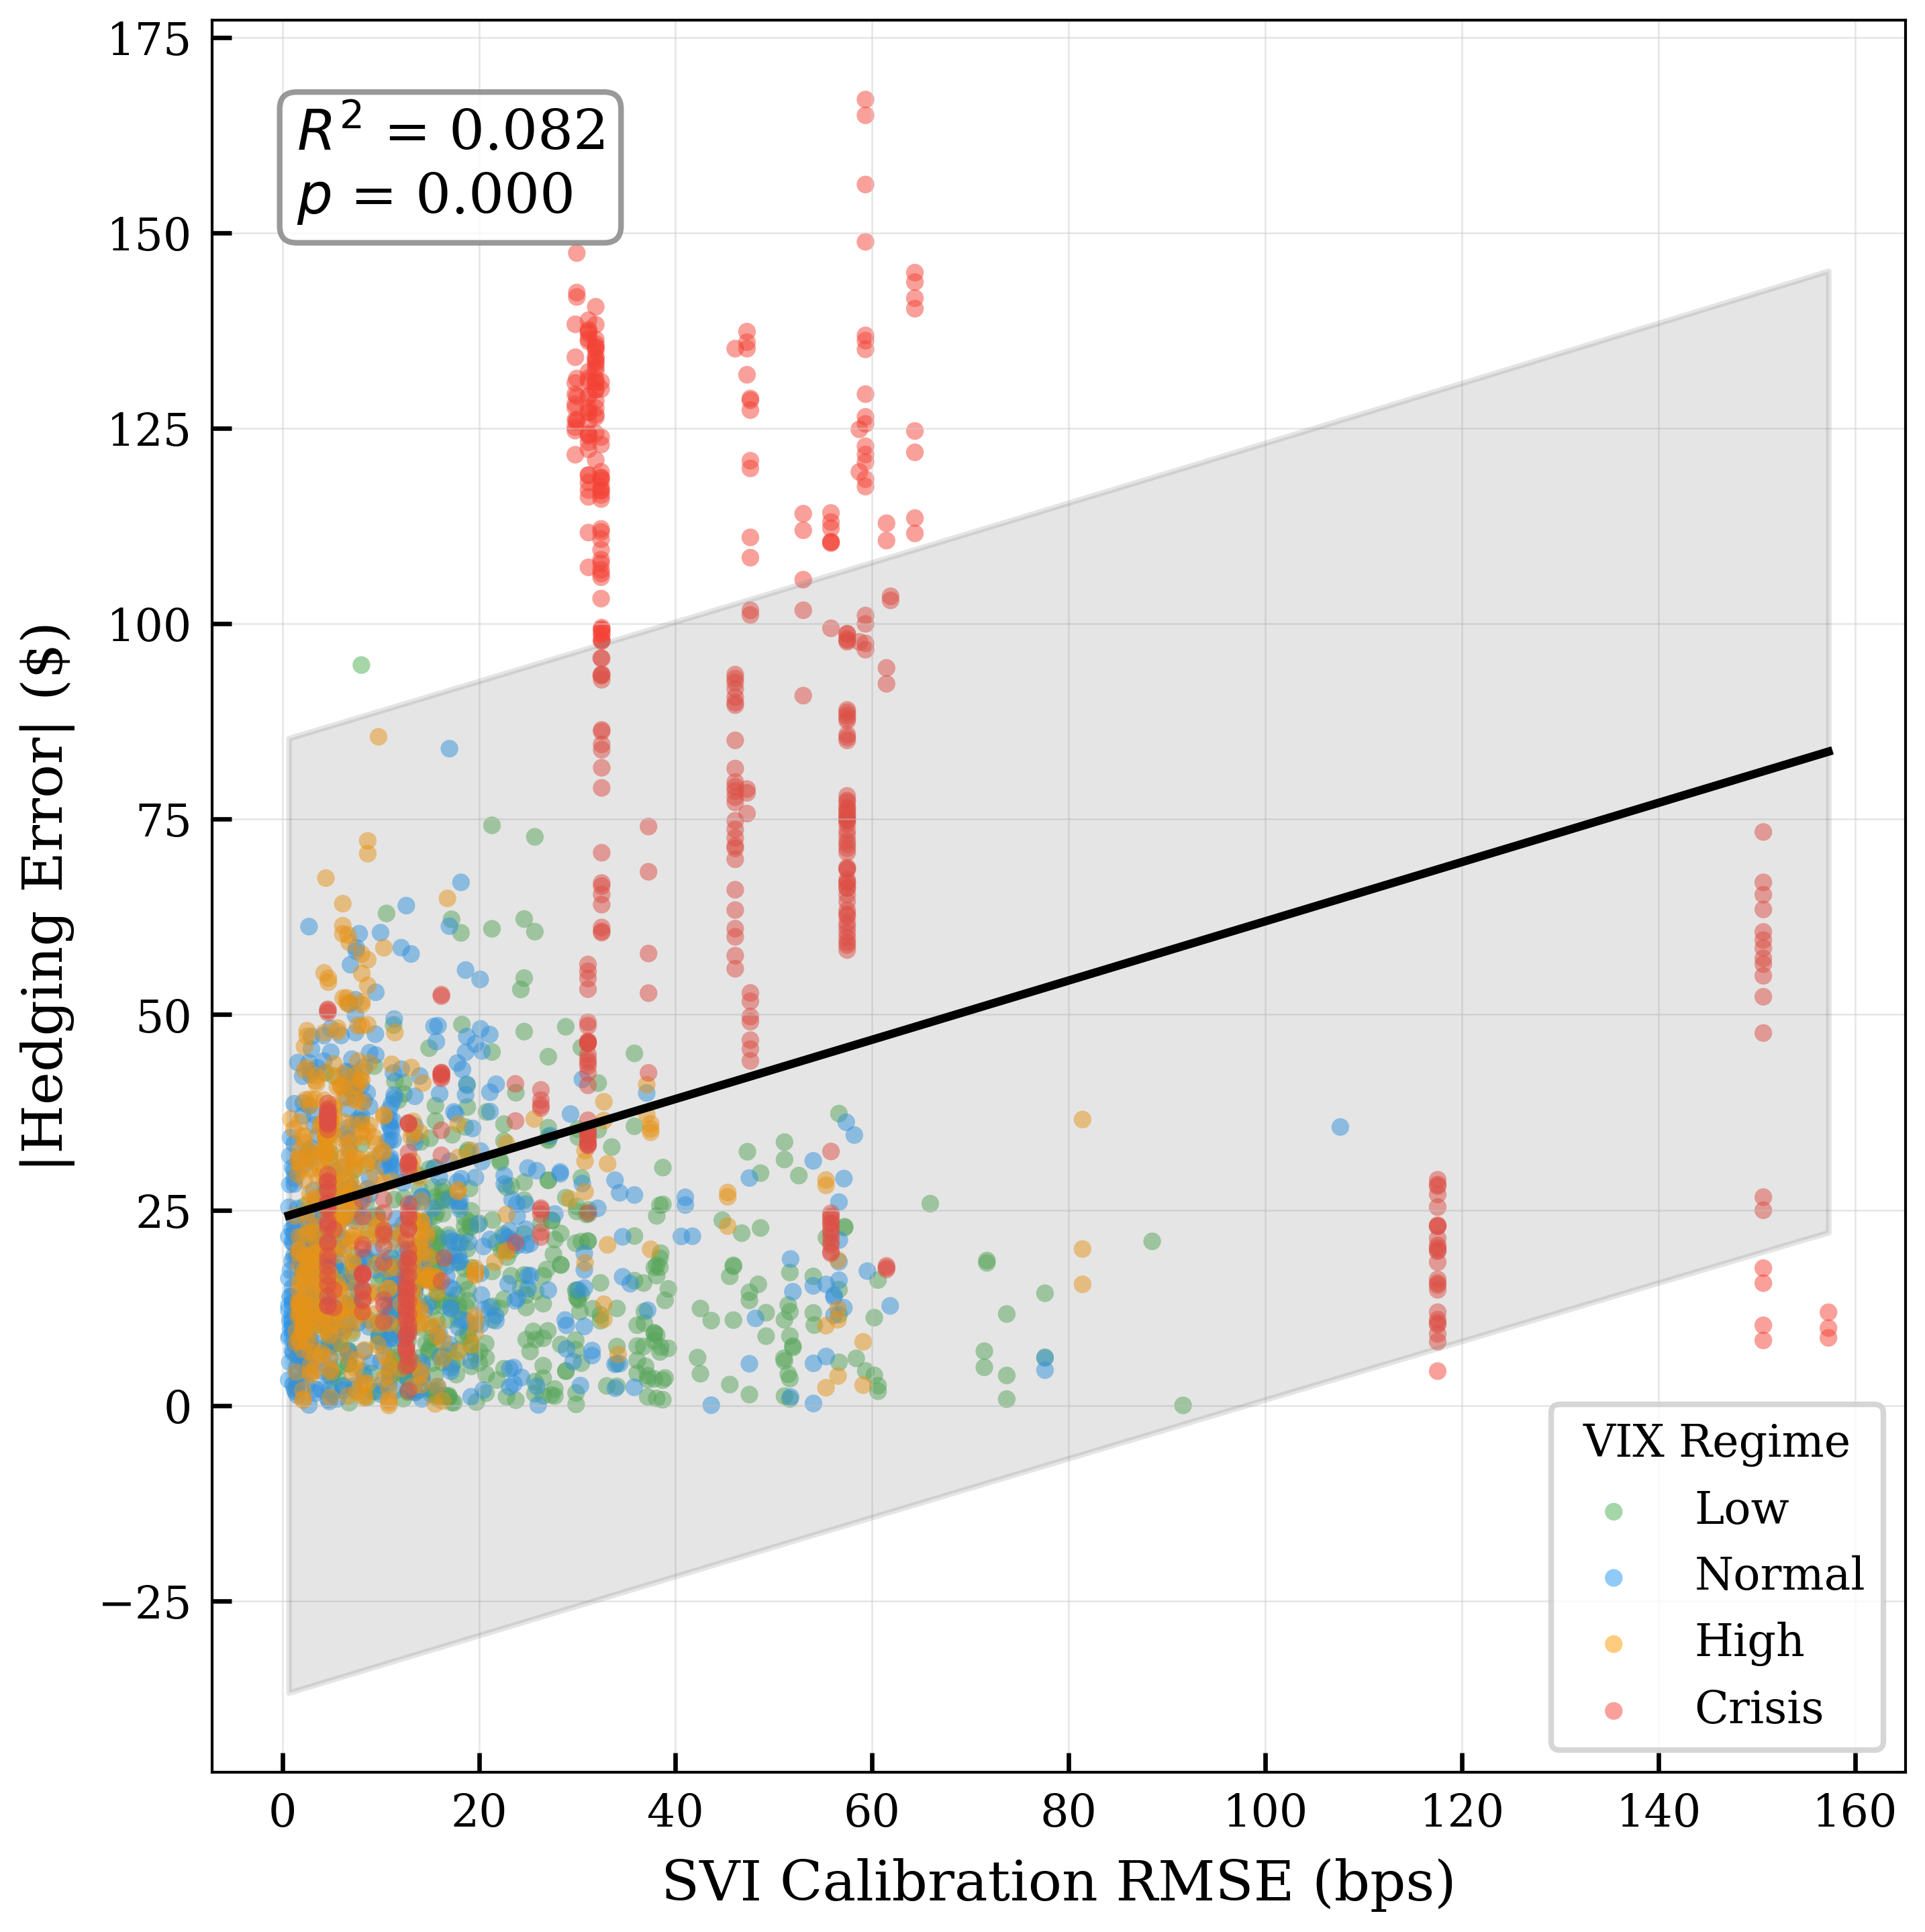
\includegraphics[width=\textwidth]{fig8_svi_vs_error.png}
\caption{SVI calibration RMSE (bps) versus absolute hedging error for SVI surface hedging. Each point is one option. The OLS regression line suggests a weak positive relationship, indicating that calibration noise propagates into hedging error.}
\label{fig:svi_hedge}
\end{figure}

The scatter reveals a weak but positive relationship: options hedged during periods of high SVI calibration error tend to have larger hedging errors. This supports the interpretation that SVI's aggregate underperformance is partly driven by calibration noise---when the SVI fit is poor, the resulting implied volatilities are more harmful than helpful.

\subsection{Delta-Gamma Hedging}
\label{sec:delta_gamma}

To complement the empirical backtest, I validate the delta-gamma hedging extension using simulated paths, consistent with the Monte Carlo framework described in Section~\ref{sec:pricing}. Delta-only hedging leaves the portfolio exposed to gamma risk: large moves in the underlying generate hedging errors proportional to $\frac{1}{2}\Gamma(\Delta S)^2$ (Equation~\ref{eq:discrete_error}). Delta-gamma hedging neutralizes this exposure by adding a second option to the hedge portfolio.

\subsubsection{Setup}

Consider a short position in a call option with strike $K_1$ on the SPX index. A delta-gamma hedge supplements the underlying position with a second option struck at $K_2$:
\begin{equation}
    \Pi = -V_1 + \Delta_{\Pi} \cdot S + n_2 \cdot V_2,
    \label{eq:dg_portfolio}
\end{equation}
where $V_1$ is the target option, $V_2$ is the hedging instrument (strike $K_2 = 110$), $n_2$ is chosen to zero out portfolio gamma, and $\Delta_{\Pi}$ is the residual delta after the gamma offset. The gamma-neutralizing quantity is:
\begin{equation}
    n_2 = -\frac{\Gamma_1}{\Gamma_2}, \qquad \Delta_{\Pi} = \Delta_1 - n_2 \cdot \Delta_2.
    \label{eq:gamma_neutral}
\end{equation}
At each rebalancing date, both $n_2$ and $\Delta_{\Pi}$ are recalculated to maintain simultaneous delta and gamma neutrality.

\subsubsection{Simulation Design}

I simulate 50,000 geometric Brownian motion paths using antithetic variates for variance reduction. The underlying starts at $S_0 = 100$ with $\sigma = 0.20$, $r = 0.05$, and $q = 0$. The target option is an ATM call ($K_1 = 100$) with 30 days to expiry, rebalanced daily. The hedging instrument is a call struck at $K_2 = 110$.

\subsubsection{Results}

Table~\ref{tab:delta_gamma} compares delta-only and delta-gamma hedging across the 50,000 simulated paths.

\begin{table}[H]
\centering
\caption{Delta-only versus delta-gamma hedging on 50,000 simulated GBM paths. The second hedging instrument is a call with strike $K_2 = 110$. Std and percentiles are in dollars.}
\label{tab:delta_gamma}
\begin{tabular}{lcc}
\toprule
Metric & Delta-Only & Delta-Gamma \\
\midrule
P\&L Std (\$)          & 0.44 & 0.24 \\
95\% Range             & $[-0.92, +0.90]$ & $[-0.35, +0.32]$ \\
Std Reduction          & ---  & 46\% \\
\bottomrule
\end{tabular}
\end{table}

Delta-gamma hedging reduces P\&L standard deviation by 46\%, from \$0.44 to \$0.24. The 95\% range compresses from $[-\$0.92, +\$0.90]$ to $[-\$0.35, +\$0.32]$, a factor-of-2.6 reduction in tail exposure. This improvement is consistent with the P\&L attribution results in Section~\ref{sec:pnl_attribution}: since the discrete rebalancing error scales with $\Gamma$, neutralizing gamma directly eliminates the dominant source of hedging variance in calm markets.

These simulation results motivate a natural extension: applying delta-gamma hedging to the empirical SPX backtest. The key challenge is identifying a liquid second hedging instrument for each target option---a question I leave for future work (Section~\ref{sec:conclusion}). The 46\% variance reduction observed in simulation represents an upper bound, as real-world implementation would face transaction costs from maintaining positions in two options and potential illiquidity in the hedging instrument.

\subsection{Statistical Significance}
\label{sec:stat_tests}

Table~\ref{tab:stat_tests} reports formal statistical tests comparing each volatility input to the flat BSM benchmark.

\begin{table}[H]
\centering
\caption{Statistical tests comparing alternative volatility inputs to the Flat BSM benchmark. Paired $t$-test is on absolute hedging errors; $F$-test is on hedging error variances; Diebold--Mariano test is on squared errors.}
\label{tab:stat_tests}
\begin{tabular}{lcccccc}
\toprule
Comparison & $t$ & $p_t$ & $F$ & $p_F$ & DM & $p_{\text{DM}}$ \\
\midrule
SVI Surface vs.\ Flat BSM & 5.64  & $< 0.001$ & 1.20 & $< 0.001$ & 10.13 & $< 0.001$ \\
RV (CC) vs.\ Flat BSM     & $-4.51$ & $< 0.001$ & 0.89 & 0.008    & $-3.34$ & $< 0.001$ \\
\bottomrule
\end{tabular}
\end{table}

Both comparisons are highly significant:
\begin{itemize}
    \item \textbf{SVI vs.\ Flat BSM:} SVI is significantly \textit{worse} on all three tests. The $F$-statistic of 1.20 indicates SVI hedging error variance is 20\% larger than flat BSM ($p < 0.001$). The positive $t$-statistic indicates larger mean absolute errors. The large positive DM statistic indicates larger mean squared errors.
    \item \textbf{RV (CC) vs.\ Flat BSM:} CC is significantly \textit{better}. The $F$-statistic of 0.89 indicates 11\% lower variance ($p = 0.008$). The negative $t$ and DM statistics indicate smaller absolute and squared errors.
\end{itemize}


% =============================================================================
% CHAPTER 6: DISCUSSION AND IMPLICATIONS
% =============================================================================
\section{Discussion and Implications}
\label{sec:discussion}

\subsection{Why Does the Smile Hurt?}

The central puzzle of this thesis is why SVI surface IV---which contains strictly more information than flat ATM IV---produces worse hedging outcomes in aggregate. I offer three explanations.

\textbf{Calibration noise.} Every SVI calibration introduces estimation error. The five-parameter optimization is sensitive to the strike grid, bid-ask spreads, and outliers. While the median RMSE of 19.5 bps is good, it is non-zero, and this error propagates into the hedge delta through $d_1$. In contrast, flat ATM IV uses a single observed market price with zero calibration error.

\textbf{Interpolation artifacts.} To make the calibration tractable, I calibrate every 5th trading day and interpolate parameters between calibration dates. This temporal smoothing may introduce stale smile information on non-calibration dates, producing hedge deltas that are responsive to yesterday's smile rather than today's.

\textbf{The smile is informative but noisy.} The moneyness-conditional results (Table~\ref{tab:best_vol}) show that SVI \textit{does} help for OTM calls, where the smile slope is steepest and the informational content of strike-specific IV is highest. But for other option types, the noise outweighs the signal. This interpretation is consistent with the SVI RMSE regression (Figure~\ref{fig:svi_hedge}): when calibration quality is high, SVI hedging tends to be better.

\subsection{For Practitioners: Which Vol to Hedge With}

The answer depends on what you trade:

\begin{itemize}
    \item \textbf{ATM options:} Use flat BSM IV for short-dated, RV (Yang--Zhang) for medium and long-dated. The smile adds nothing at the money.
    \item \textbf{OTM calls:} Use SVI surface IV. The upside smile slope contains hedgeable information (Gain of 6--12\% vs.\ flat BSM).
    \item \textbf{OTM puts:} Use close-to-close realized vol. The skew premium makes implied-based deltas systematically biased, and a backward-looking estimator provides a better anchor.
    \item \textbf{Crisis periods:} No method works well. Focus on position sizing and gamma management rather than delta precision.
\end{itemize}

\subsection{For Vol Desks: Is SVI Calibration Worth It?}

For pure delta hedging, SVI calibration does not pay for itself in aggregate. However, SVI calibration serves other purposes beyond hedging---pricing exotic derivatives, monitoring arbitrage-free conditions, and interpolating the surface for risk management. The hedging results suggest that desks should not use raw SVI-calibrated IVs as delta inputs without a regime-conditional filter.

A practical improvement would be a moneyness-conditional strategy: use SVI deltas for the OTM call book and flat BSM or realized vol deltas for everything else. The estimated Gain from such a conditional approach, based on the cell-level results in Table~\ref{tab:best_vol}, would exceed any single-input strategy.

\subsection{For Risk Managers: What to Monitor}

The P\&L decomposition (Section~\ref{sec:pnl_attribution}) reveals that higher-order residuals---not discrete rebalancing error or vol misspecification---dominate hedging P\&L variance across all regimes. This suggests that risk managers should focus on:
\begin{enumerate}
    \item \textbf{Gamma exposure:} All three P\&L components scale with $\Gamma$. Reducing net gamma reduces all sources of hedging error.
    \item \textbf{Vanna and volga risk:} The large residual component likely captures smile dynamics (vanna: $\partial\Delta/\partial\sigma$) and convexity in the vol-of-vol (volga). These are particularly important during regime transitions.
    \item \textbf{Jump risk:} The COVID-19 period shows that large gap moves overwhelm any delta-hedging approach, regardless of the volatility input.
\end{enumerate}

\subsection{Connection to Prior Work}

These findings complement \citet{Hull2017}, who report Gains of 2--10\% for their minimum-variance delta approach. My close-to-close RV result (Gain = $+5.8\%$) falls within this range, achieved through a simpler method. The regime dependence echoes \citet{Alexander2012}, who show that smile-adjusted deltas are less reliable in high-volatility environments. My SVI results quantify this: the smile helps during Normal and High VIX (Gain = $+0.8\%$ and $+3.7\%$) but hurts during Low and Crisis regimes.


% =============================================================================
% CHAPTER 7: LIMITATIONS, FUTURE WORK, AND CONCLUSION
% =============================================================================
\section{Limitations, Future Work, and Conclusion}
\label{sec:conclusion}

\subsection{Limitations}

Several limitations should be noted when interpreting these results:

\begin{enumerate}
    \item \textbf{SPX-specific.} The results apply to European-style S\&P~500 index options. Single-stock options, which face earnings jumps, dividends, and lower liquidity, may produce different rankings.

    \item \textbf{Daily rebalancing only.} I rebalance at the daily close, matching the frequency of OptionMetrics data. Intraday rebalancing or more frequent adjustment could change the relative performance of different volatility inputs, particularly for short-dated options where gamma is large.

    \item \textbf{European options only.} SPX options are European-style, eliminating early-exercise complications. American-style options on single stocks would require adjusting the hedging framework for early exercise probability.

    \item \textbf{No stochastic volatility model comparison.} I compare five BSM-based volatility inputs but do not test hedge ratios from stochastic volatility models (Heston, SABR). These models would produce different deltas that account for vol-of-vol and mean reversion.

    \item \textbf{Sample period specific.} The 2019--2024 period includes the COVID-19 crash, which is an extreme outlier. Results may differ in a period without such large dislocations.

    \item \textbf{Transaction costs ignored.} All hedging is frictionless. In practice, more frequent rebalancing (which benefits realized vol methods) would incur greater transaction costs that could offset the hedging improvement.

    \item \textbf{SVI calibration choices.} The thinning to every 5th day and the parameter interpolation scheme are pragmatic choices that affect SVI hedging quality. Daily calibration or more sophisticated interpolation could improve SVI's performance.
\end{enumerate}

\subsection{Future Work}

Several extensions could build on this framework:

\begin{enumerate}
    \item \textbf{Single-stock options.} Extending the analysis to options on individual equities such as AAPL, NVDA, and TSLA would test whether the findings generalize to American-style options with earnings-driven dynamics, discrete dividends, and higher idiosyncratic volatility. The existing framework is directly portable with minor adjustments for early exercise.

    \item \textbf{Stochastic volatility model comparison.} Computing hedge ratios from calibrated Heston or SABR models would test whether model-based deltas outperform the BSM deltas with alternative volatility inputs studied here.

    \item \textbf{Deep hedging benchmark.} Recent work on neural-network-based hedging strategies \citep{Buehler2019} provides a model-free benchmark. Comparing the five volatility inputs against a deep hedging approach would quantify how much of the hedging error is reducible in principle.

    \item \textbf{Intraday rebalancing.} Using intraday data to rebalance multiple times per day would reduce the discrete rebalancing error component and could change the relative rankings, particularly for gamma-sensitive short-dated options.

    \item \textbf{VRP-conditioned hedging.} The variance risk premium (implied minus realized vol) is a known predictor of future realized vol. A hedging strategy that dynamically selects the volatility input based on the current VRP could outperform any static choice.

    \item \textbf{Arbitrage-free SVI calibration.} Using the SSVI parameterization of \citet{Gatheral2014} or penalized optimization that explicitly enforces the Durrleman condition could improve both calibration quality and hedging outcomes, particularly for the 31.4\% of slices that currently exhibit butterfly arbitrage violations.
\end{enumerate}

\subsection{Conclusion}

This thesis provides the first empirical evaluation of SVI-calibrated implied volatility as a delta-hedging input on real S\&P~500 index options. The results challenge three common assumptions.

First, more information does not automatically improve hedging. The SVI surface, despite encoding the full implied volatility smile with high calibration quality (median RMSE of 19.5 bps), produces 9.4\% higher hedging error variance than flat ATM implied volatility. The calibration noise embedded in the five-parameter SVI fit outweighs the informational benefit of strike-specific volatilities for most option types.

Second, statistical efficiency in volatility estimation does not translate into hedging efficiency. The simple close-to-close realized volatility estimator, which uses only closing prices, outperforms both the Parkinson and Yang--Zhang estimators, which incorporate intraday range information. For hedging purposes, smoothness (low sensitivity to intraday noise) appears more valuable than efficiency (low estimation variance under GBM).

Third, and most importantly, the optimal volatility input is strongly dependent on option moneyness and market regime. SVI surface IV reduces hedging error for out-of-the-money calls by 6--12\%, where the smile slope carries genuine hedgeable information. Realized volatility dominates for out-of-the-money puts, where the skew premium makes implied-based deltas biased. No single input wins everywhere, suggesting that a moneyness-conditional hedging strategy---using different volatility inputs for different regions of the option space---would outperform any static approach.

These findings have practical implications for options desks, risk managers, and researchers. For practitioners, they provide concrete guidance on which volatility to hedge with and when. For the SVI literature, they fill a gap between calibration quality and economic outcomes. For the broader delta-hedging literature, they demonstrate that the choice of volatility input matters at least as much as the choice of hedging model---and that the answer is not one-size-fits-all.


% =============================================================================
% REFERENCES
% =============================================================================
\newpage
\bibliographystyle{plainnat}

\begin{thebibliography}{99}

\bibitem[Alexander et~al.(2012)]{Alexander2012}
Alexander, C., Kaeck, A., and Nogueira, L.~M. (2012).
\newblock Model-free hedge ratios and scale-invariant models.
\newblock \textit{Journal of Banking \& Finance}, 36(12):3267--3282.

\bibitem[Bakshi et~al.(1997)]{Bakshi1997}
Bakshi, G., Cao, C., and Chen, Z. (1997).
\newblock Empirical performance of alternative option pricing models.
\newblock \textit{The Journal of Finance}, 52(5):2003--2049.

\bibitem[Black and Scholes(1973)]{Black1973}
Black, F. and Scholes, M. (1973).
\newblock The pricing of options and corporate liabilities.
\newblock \textit{Journal of Political Economy}, 81(3):637--654.

\bibitem[B{\"u}hler et~al.(2019)]{Buehler2019}
B{\"u}hler, H., Gonon, L., Teichmann, J., and Wood, B. (2019).
\newblock Deep hedging.
\newblock \textit{Quantitative Finance}, 19(8):1271--1291.

\bibitem[Diebold and Mariano(1995)]{DieboldMariano1995}
Diebold, F.~X. and Mariano, R.~S. (1995).
\newblock Comparing predictive accuracy.
\newblock \textit{Journal of Business \& Economic Statistics}, 13(3):253--263.

\bibitem[Durrleman(2005)]{Durrleman2005}
Durrleman, V. (2005).
\newblock \textit{From Implied to Spot Volatilities}.
\newblock PhD thesis, Princeton University.

\bibitem[El~Karoui et~al.(1998)]{ElKaroui1998}
El~Karoui, N., Jeanblanc-Picqu{\'e}, M., and Shreve, S.~E. (1998).
\newblock Robustness of the {Black} and {Scholes} formula.
\newblock \textit{Mathematical Finance}, 8(2):93--126.

\bibitem[Gatheral(2004)]{Gatheral2004}
Gatheral, J. (2004).
\newblock A parsimonious arbitrage-free implied volatility parameterization with application to the valuation of volatility derivatives.
\newblock Presentation at Global Derivatives \& Risk Management, Madrid.

\bibitem[Gatheral and Jacquier(2014)]{Gatheral2014}
Gatheral, J. and Jacquier, A. (2014).
\newblock Arbitrage-free {SVI} volatility surfaces.
\newblock \textit{Quantitative Finance}, 14(1):59--71.

\bibitem[Hagan et~al.(2002)]{Hagan2002}
Hagan, P.~S., Kumar, D., Lesniewski, A.~S., and Woodward, D.~E. (2002).
\newblock Managing smile risk.
\newblock \textit{Wilmott Magazine}, September:84--108.

\bibitem[Heston(1993)]{Heston1993}
Heston, S.~L. (1993).
\newblock A closed-form solution for options with stochastic volatility with applications to bond and currency options.
\newblock \textit{The Review of Financial Studies}, 6(2):327--343.

\bibitem[Hull(2021)]{Hull2018}
Hull, J.~C. (2021).
\newblock \textit{Options, Futures, and Other Derivatives}.
\newblock Pearson, 11th edition.

\bibitem[Hull and White(2017)]{Hull2017}
Hull, J.~C. and White, A. (2017).
\newblock Optimal delta hedging for options.
\newblock \textit{Journal of Banking \& Finance}, 82:180--190.

\bibitem[Merton(1973)]{Merton1973}
Merton, R.~C. (1973).
\newblock Theory of rational option pricing.
\newblock \textit{The Bell Journal of Economics and Management Science}, 4(1):141--183.

\bibitem[Parkinson(1980)]{Parkinson1980}
Parkinson, M. (1980).
\newblock The extreme value method for estimating the variance of the rate of return.
\newblock \textit{Journal of Business}, 53(1):61--65.

\bibitem[Shu and Zhang(2006)]{Shu2006}
Shu, J. and Zhang, J.~E. (2006).
\newblock Testing range estimators of historical volatility.
\newblock \textit{Journal of Futures Markets}, 26(3):297--313.

\bibitem[Storn and Price(1997)]{Storn1997}
Storn, R. and Price, K. (1997).
\newblock Differential evolution---a simple and efficient heuristic for global optimization over continuous spaces.
\newblock \textit{Journal of Global Optimization}, 11(4):341--359.

\bibitem[Taleb(1997)]{Taleb1997}
Taleb, N.~N. (1997).
\newblock \textit{Dynamic Hedging: Managing Vanilla and Exotic Options}.
\newblock John Wiley \& Sons.

\bibitem[Yang and Zhang(2000)]{Yang2000}
Yang, D. and Zhang, Q. (2000).
\newblock Drift-independent volatility estimation based on high, low, open, and close prices.
\newblock \textit{Journal of Business}, 73(3):477--492.

\end{thebibliography}

\end{document}
